\def\GRAPHPATH{graphics}

\ifdefined\HANDOUT
  \documentclass[handout,aspectratio=1610,dvipsnames]{beamer}
  \def\GRAPHPATH{graphics}
\else
  \documentclass[aspectratio=1610,dvipsnames]{beamer}
\fi

\input{localpackages.tex}
\input{localcommands.tex}

\ifdefined\TITLE
  \title[Logik/Semantik | \letterssub{\TITLE}]{Minimale Logik und Semantik für die Sprachphilosophie\\\letterssub{\TITLE}}
\else
  \title[Logik/Semantik]{Minimale Logik und Semantik für die Sprachphilosophie}
\fi

\author{Roland Schäfer}
\institute[FSU Jena]{Institut für Germanistische Sprachwissenschaft\\Friedrich-Schiller-Universität Jena}
\date[\today]{\grau{Stets aktuelle Fassungen: \url{https://github.com/rsling/VL-Semantik}}}

\begin{document}

\begingroup
  \setbeamertemplate{navigation symbols}{}
  \begin{frame}[noframenumbering,plain,allowframebreaks]
   \titlepage
  \end{frame}
  \begin{frame}{Inhalt}
    \centering
    \begin{minipage}{0.8\textwidth}
        \begin{multicols}{2}
          \tableofcontents
        \end{multicols}
    \end{minipage}
  \end{frame}
\endgroup

\ifdefined\TITLE
  \input{includes/\TITLE}
\else
  \section[Inferenz und Bedeutung]{Inferenz und Bedeutung}
  \let\woopsi\section\let\section\subsection\let\subsection\subsubsection
  
\section{Organisation}

\begin{frame}
  {Literatur | Einführungen}
  \onslide<+->
  \onslide<+->
  Die folgenden drei Bücher sind die Grundlage der Vorträge:\\
  \Zeile
  \begin{itemize}[<+->]
    \item \alert{\citet{ChierchiaMcconnellginet2000}} | GB-orientiert, nur die Kapitel von Chierchia
    \item \alert{\citet{DowtyEa1981}} | Tolle Montague-Einführung von seinen Schülern
    \item \alert{\citet{ParteeEa1990}} | Wichtige Grundlagen (Algebra, Logik), viele Druckfehler
  \end{itemize}
  \onslide<+->
  \centering 
  \large
  \Zeile
  \rot{Die auf den Folien angegebenen Teile dieser Bücher sollten\\
  für die Prüfungen durchgearbeitet werden. Das heißt natürlich nicht,\\
  dass Sie alles auswendig lernen sollen. Die Folien geben die Hinweise,\\
  was aus den Texten wichtig ist, sind aber nicht selbsterklärend.}
\end{frame}

\begin{frame}
  {Literatur | weitere Empfehlungen}
  \onslide<+->
  \begin{itemize}[<+->]
    \item \alert{\citet{Bucher1998}} | Lesbare Logik-Einführung auf Deutsch
    \item \alert{\citet{Carpenter1997}} | Prima Hardcore-Einführung mit Kategorialgrammatik
    \item \alert{\citet{Gutzmann2019}} | Aktuelle Einführung auf Deutsch
  \end{itemize}
\end{frame}


\begin{frame}
  {Semesterplan und Lernen für die Prüfung}
  \onslide<+->
  \onslide<+->
  \centering 
  \alert{\large Hinweis zum Lernen}\\
  \Halbzeile
  \begin{itemize}[<+->]
    \item Wir haben es hier mit anspruchsvollem Material zu tun.
    \item Nur so ergibt meiner Meinung nach formale Semantik Sinn,\\
      und irgendwelche weichgespülten Einführungen sind grob fahrlässig.
    \item Daher gilt aber: Wenn Sie nicht von Anfang an lernen,\\
      wird es sehr wahrscheinlich gegen Ende sehr schwierig!
  \end{itemize}
\end{frame}

\begin{frame}
  {Prüfungen}
  \onslide<+->
  \onslide<+->
  Einheitlicher Inhalt für alle Modul- und Examensprüfungen:\\
  \Zeile
  \begin{quote}
    Sie erhalten in der Prüfung zwei der Originaltexte zur Auswahl und müssen einen davon diskutieren und in den Seminarkontext einordnen. Dazu gibt es Leitfragen, über die ich auf Basis des Seminarverlaufs entscheide.
  \end{quote}
  \Zeile
  \onslide<+->
  \grau{Hausarbeiten nach Absprache.}
\end{frame}

\begin{frame}
  {Die unausweichliche Frage nach ein paar Wochen \visible<2->{| \rot{WTF???}}}
  \onslide<+->
  \onslide<+->
  \onslide<+->
  "`Wozu brauchen wir das denn?"'\\
  \Halbzeile
  \begin{itemize}[<+->]
    \item Nicht zu leugnende \alert{logische Eigenschaften von Sprache}
    \item Kleiner Einblick in deren \alert{technisch sehr aufwendige Beschreibung}
      \Halbzeile
    \item Wichtige Lernziele
      \begin{itemize}[<+->]
        \item Realistische Einschätzung \alert{eigener semantischer Intuitionen}
        \item Erkennen der \alert{Grenzen der Möglichkeiten von Logik} in der Analyse von Sprache
        \item Für zukünftige Forschende | \alert{Grundausbildung in formaler Semantik unabdinglich}
      \end{itemize}
  \end{itemize}
\end{frame}

\section{Schlussfolgern}

\begin{frame}
  {Was folgt logisch?}
  \onslide<+->
  \onslide<+->
  Fallen Ihnen logische Schlussfolgerungen aus diesen Aussagen ein?\\
  \Halbzeile
  \begin{itemize}[<+->]
    \item Das Semester hat begonnen.
    \item Olha hat einen sehr leichten ukrainischen Akzent.
    \item Entweder regnet es gerade, oder die Wasserleitung ist gebrochen.
    \item Es regnet, oder die Wasserleitung ist gebrochen. Es regnet seit zwei Stunden.
    \item Falls der Dänemark-Urlaub ausfällt, fahre ich eine Woche zu meinen Eltern.\\
      Der Dänemark-Urlaub fällt aus.
    \item Wenn es regnet, wird die Straße nass. Die Straße ist nicht nass.
    \item Es ist nicht der Fall, dass der WANG PC keine Festplatten unterstützt hat.
  \end{itemize}
\end{frame}

\begin{frame}
  {Folgt B aus A?} % Sätze
  \onslide<+->
  \begin{itemize}[<+->]
    \item A: Ein blauer Renault fährt auf der A9 Richtung Berlin.\\
      \alert{B: Ein Renault fährt auf der A9 Richtung Berlin.}
    \item A: Ich finde Geranien abstoßend.\\
      \alert{B: Ich habe schon mindestens einmal mindestens eine Geranie gesehen.}
    \item A: Der WANG PC ist nicht IBM-kompatibel.\\
      \alert{B: Es existiert mindestens ein WANG PC.}
    \item A: Alle Menschen sind intelligent.\\
      \alert{B: Horst Lichter ist intelligent.}
    \item A: Krister hat mir seinen Volvo Amazon verkauft.\\
      \alert{B: Irgendjemand hat seinen Volvo Amazon verkauft.}
  \end{itemize}
\end{frame}

\begin{frame}
  {Folgt B aus A?} % Lexik und Grammatik
  \begin{itemize}[<+->]\small
    \item A: Entweder regnet es, oder die Wasserleitung im Bad ist gebrochen, und die Wasserleitung im Bad ist gebrochen.\\
      \alert{B: Es regnet nicht.}
    \item A: Michelle hat uns den Dobermann für eine Woche zur Pflege überlassen.\\
      \alert{B: Der Dobermann wurde uns für eine Woche zur Pflege überlassen.}
    \item A: Jan glaubt, dass seine Sendung nicht abgesetzt wird.\\
      \alert{B: Jan glaubt nicht, dass seine Sendung abgesetzt wird.}
    \item A: Falls Dr.\ Kohl jetzt wieder Kanzler der BRD ist, gibt es vermutlich jeden Tag Pfälzer Saumagen zum Abendessen.\\
      \alert{B: Es gibt einen Kanzler der BRD.}
    \item A: Ein Mensch betritt den Raum.\\
      \alert{B: Es gibt mindestens einen Menschen.}
    \item A: Ein Mensch, der die Bibel gelesen hat, begeht im Durchschnitt nicht weniger Straftaten als andere.\\
      \alert{B: Es gibt mindestens einen Menschen.}
    \item A: \textit{We don't need no education.}\\
      \alert{B: Yes, you do! You just used a double negative.}
  \end{itemize}
\end{frame}

\begin{frame}
  {Folgt B aus A?} % Stories
  \onslide<+->
  \begin{itemize}[<+->]
    \item A: Herr Sailer fährt einen Golf. Alles, was einen Golf fährt, ist entweder menschlich oder eine AI, die auf Deep Learning basiert. Es gibt keine AI, die auf Deep Learning basiert, die einen Golf fährt.\\
      \alert{B: Es gibt mindestens einen Menschen.}
      \Halbzeile
    \item A: Es gibt an der Uni Göttingen mindestens einen Dozenten, der einen Golf fährt. Manfred ist Dozent an der Uni Göttingen und Radsportler. Sein Auto ist gerade in der Werkstatt. Jeder Dozent an der Uni Göttingen fährt entweder einen Golf oder ist kein Radsportler, falls sein Auto in der Werkstatt ist.\\
      \alert{B: Manfred fährt einen Golf.}
  \end{itemize}
\end{frame}

\begin{frame}
  {Logik}
  \onslide<+->
  \onslide<+->
  \centering 
  Versuchen Sie, eine Definition des Begriffs \alert{logische Schlussfolgerung} zu geben.\\
  \onslide<+->
  \Zeile
  Wann folgt eine Aussage aus einer oder mehreren anderen Aussagen?
\end{frame}

\begin{frame}
  {Inferenz | Abduktion}
  \onslide<+->
  \onslide<+->
  Entspricht oft der "`Alltagslogik"'. Suche nach \alert{spontan plausiblen Ursachen}.\\
  \Halbzeile
  \begin{itemize}[<+->]
    \item A: Der Verdächtige hat kein Alibi, aber ein Motiv.\\
      B: Der Verdächtige ist der Täter.
    \item Ich habe so einen komischen Husten, und die Infektionszahlen steigen wieder.\\
      B: Oh mein Gott, ich habe Covid!
    \item A: Es soll eine Impfpflicht eingeführt werden.\\
      B: George Soros und Bill Gates wollen uns Mikrochips einpflanzen.
    \item A: In Mikes Büro ist um 22 Uhr noch Licht.\\
      B: Mike bereitet seine Lehrveranstaltung für morgen vor.
  \end{itemize}
  \onslide<+->
  \centering 
  \Zeile 
  \orongsch{Hochgradig gefährlich, weil nicht formalisierbar und sehr bequem.}\\
  \alert{Gleichzeitig im Alltag unentbehrlich.}\\
  \grau{\footnotesize Die meisten "`logischen"' Schlussfolgerungen von Vulkaniern sind im besten Fall Abduktionen.}
\end{frame}

\begin{frame}
  {Inferenz | Induktion}
  \onslide<+->
  \onslide<+->
  Suche nach \alert{allgemeingültigen Aussagen} aus Partikularereignissen.\\
  \Halbzeile
  \begin{itemize}[<+->]
    \item A\Sub{1}: Im Zentrum der Galaxis befindet sich ein supermassives schwarzes Loch.\\
          A\Sub{2}: Die Galaxis ist eine Galaxie.\\
          B: Im Zentrum jeder Galaxie befindet sich ein supermassives schwarzes Loch.
    \item A: Im Zentrum von 1200 Galaxien befindet sich ein supermassives schwarzes Loch.\\
          B: Im Zentrum jeder Galaxie befindet sich ein supermassives schwarzes Loch.
    \item A: Aus dieser Einmündung kam noch nie ein Auto von rechts.\\
          B: Aus dieser Einmündung wird in drei Sekunden kein Auto von rechts kommen.
  \end{itemize}
  \onslide<+->
  \Zeile 
  \centering 
  \alert{"`Besser"' als Abduktion, vor allem je mehr Partikularereignisse zugrundeliegen.}\\
  \orongsch{Kann trotzdem gewaltig daneben gehen.}\\
  \grau{\footnotesize Spielt in der Wissenschaft eine große Rolle, aber ist fundamental nicht ausreichend.}
\end{frame}

\begin{frame}
  {Inferenz | Deduktion}
  \onslide<+->
  \onslide<+->
  \alert{Prämissen} (egal, wo diese herkommen) und formale \alert{Schlussregeln}\\
  \Halbzeile
  \begin{itemize}[<+->]
    \item A\Sub{1}: Manfred ist ein Dozent an der Uni Göttingen.\\
      A\Sub{2}: Jeder Dozent an der Uni Göttingen ist ein Mensch.\\
      B: Manfred ist ein Mensch.
    \item A\Sub{1}: Entweder (wurde die Welt von einem Gebrauchtwagenhändler erschaffen) oder (Rewe verkauft keine Weetabix).\\
      A\Sub{2}: Rewe verkauft keine Weetabix.\\
      B: Die Welt wurde von einem Gebrauchtwagenhändler erschaffen.
  \end{itemize}
  \onslide<+->
  \Zeile
  \centering 
  \alert{Nur Deduktion ist Logik. Nur darum geht es in diesem Semester.}
\end{frame}

\begin{frame}
  {Ganz trivial ist das nicht \ldots}
  \onslide<+->
  \onslide<+->
    A: Herr Sailer fährt einen Golf. Alles, was einen Golf fährt, ist entweder menschlich oder eine AI, die auf Deep Learning basiert. Es gibt keine AI, die auf Deep Learning basiert, die einen Golf fährt.\\
    \alert{B: Es gibt mindestens einen Menschen.}\\
    \onslide<+->
    \Halbzeile
    Hier ist der Beweis:\\
    \onslide<+->
    \Halbzeile
    \centering
    \scalebox{0.8}{\begin{tabular}[h]{rll}
      1  & $G(s)$                                          & \\
      2  & $(\forall x)[(G(x)\rightarrow M(x)\vee A(x)]$   & \\
      3  & $\neg(\exists y)[A(y)\wedge G(y)]$              & $\vdash(\exists z)M(z)$  \\
      \cline{1-3}
      4  & $(\forall y)\neg[A(y)\wedge G(y)]$              & 3,QN \\
      5  & $(\forall y)[\neg A(y)\vee\neg G(y)]$           & 4,DeM \\
      6  & $(\forall y)[G(y)\rightarrow \neg A(y)]$        & 5,Komm.,Impl. \\
      7  & $G(m)\rightarrow \neg A(m)$                     & 6,$-\forall(1)$ \\
      8  & $\neg A(m)$                                     & 1,7,MP \\
      9  & $G(m)\rightarrow M(m)\vee A(m)$                 & 2,$-\forall(1)$ \\
      10 & $M(m)\vee A(m)$                                 & 1,9,MP \\
      11 & $M(m)$                                          & 8,10,DS \\
      12 & $(\exists z)M(z)$                               & 11,$+\exists$ $\blacksquare$ \\
    \end{tabular}}
\end{frame}

\section{Grundfragen der Semantik}

\begin{frame}
  {Semantikbegriff in diesem Seminar}
  \onslide<+->
  \onslide<+->
  Es dreht sich alles um die Beziehung von Sprache zur Welt!\\
  \Zeile
  \begin{itemize}[<+->]
    \item Auf welche Klassen von Objekten \alert{referieren} welche Klassen von Ausdrücken?
    \item Wann sind Sätze wahr? (auch als Phänomen der \alert{Referenz}!)
    \item Wie verhält sich die logische Struktur von Sätzen zu ihrem Informationsgehalt?
    \item Wie können Sätze eindeutig interpretiert werden,\\
      auch wenn sie mehrere Lesarten haben?
  \end{itemize}
\end{frame}

\section{Programmatisches Schlussbild}

\begin{frame}
  {Programmatisches Schlussbild | Exkurs I}
  \onslide<+->
  \onslide<+->
  \alert{Kognition}\\
  \Viertelzeile
  \begin{itemize}[<+->]
    \item basierend auf Ähnlichkeiten von wahrgenommenen Objekten
    \item optimiert für schnelle Mustererkennung \alert{in allen Bereichen}
    \item unscharfe Klassenbildung und Segmentierung der Ontologie
    \item parallele Verarbeitung (meistens mehrere Areale beteiligt)
  \end{itemize}
  \Halbzeile 
  \onslide<+->
  \alert{Symbolische Systeme}\\
  \Viertelzeile
  \begin{itemize}[<+->]
    \item diskrete Symbole, wohldefinierte Semantik
    \item scharf getrennte Klassen von Symbolen
    \item eindeutige Referenz auf ontologische Objekte
    \item intrinsische (nicht emergente) logische Eigenschaften\\
      \grau{(Axiomatik, Schlussregeln usw.)}
    \item sequentielle Verarbeitung\slash statische Deklaration\\
      \grau{(\zB Python oder PROLOG; parallele Verarbeitung immer linearisierbar)}
  \end{itemize}
\end{frame}

\begin{frame}
  {Programmatisches Schlussbild | Exkurs II}
  \onslide<+->
  \onslide<+->
  Klassisches kognitives Modell: \alert{Prototypentheorie} \grau{\citep{Rosch1973}}\\
  \onslide<+->
  \Zeile
  \alert{Diskretes Symbol}: \gruen{Vogel} \onslide<+-> \ldots\ und demgegenüber \ldots\\
  \onslide<+->
  \alert{Graduelles kognitives Konzept} basierend auf Ähnlichkeiten\slash Prototypen:\\
  \onslide<+->
  \Halbzeile
  \begin{minipage}{0.9\textwidth}
  \centering
    $\vcenter{\hbox{\includegraphics[width=0.4\textwidth]{\GRAPHPATH/spatz}}}$
    \onslide<+->
    \hspace*{0.025\textwidth}>\hspace*{0.025\textwidth}
    $\vcenter{\hbox{\includegraphics[width=0.25\textwidth]{\GRAPHPATH/kolibri}}}$
    \onslide<+->
    \hspace*{0.025\textwidth}>\hspace*{0.025\textwidth}
    $\vcenter{\hbox{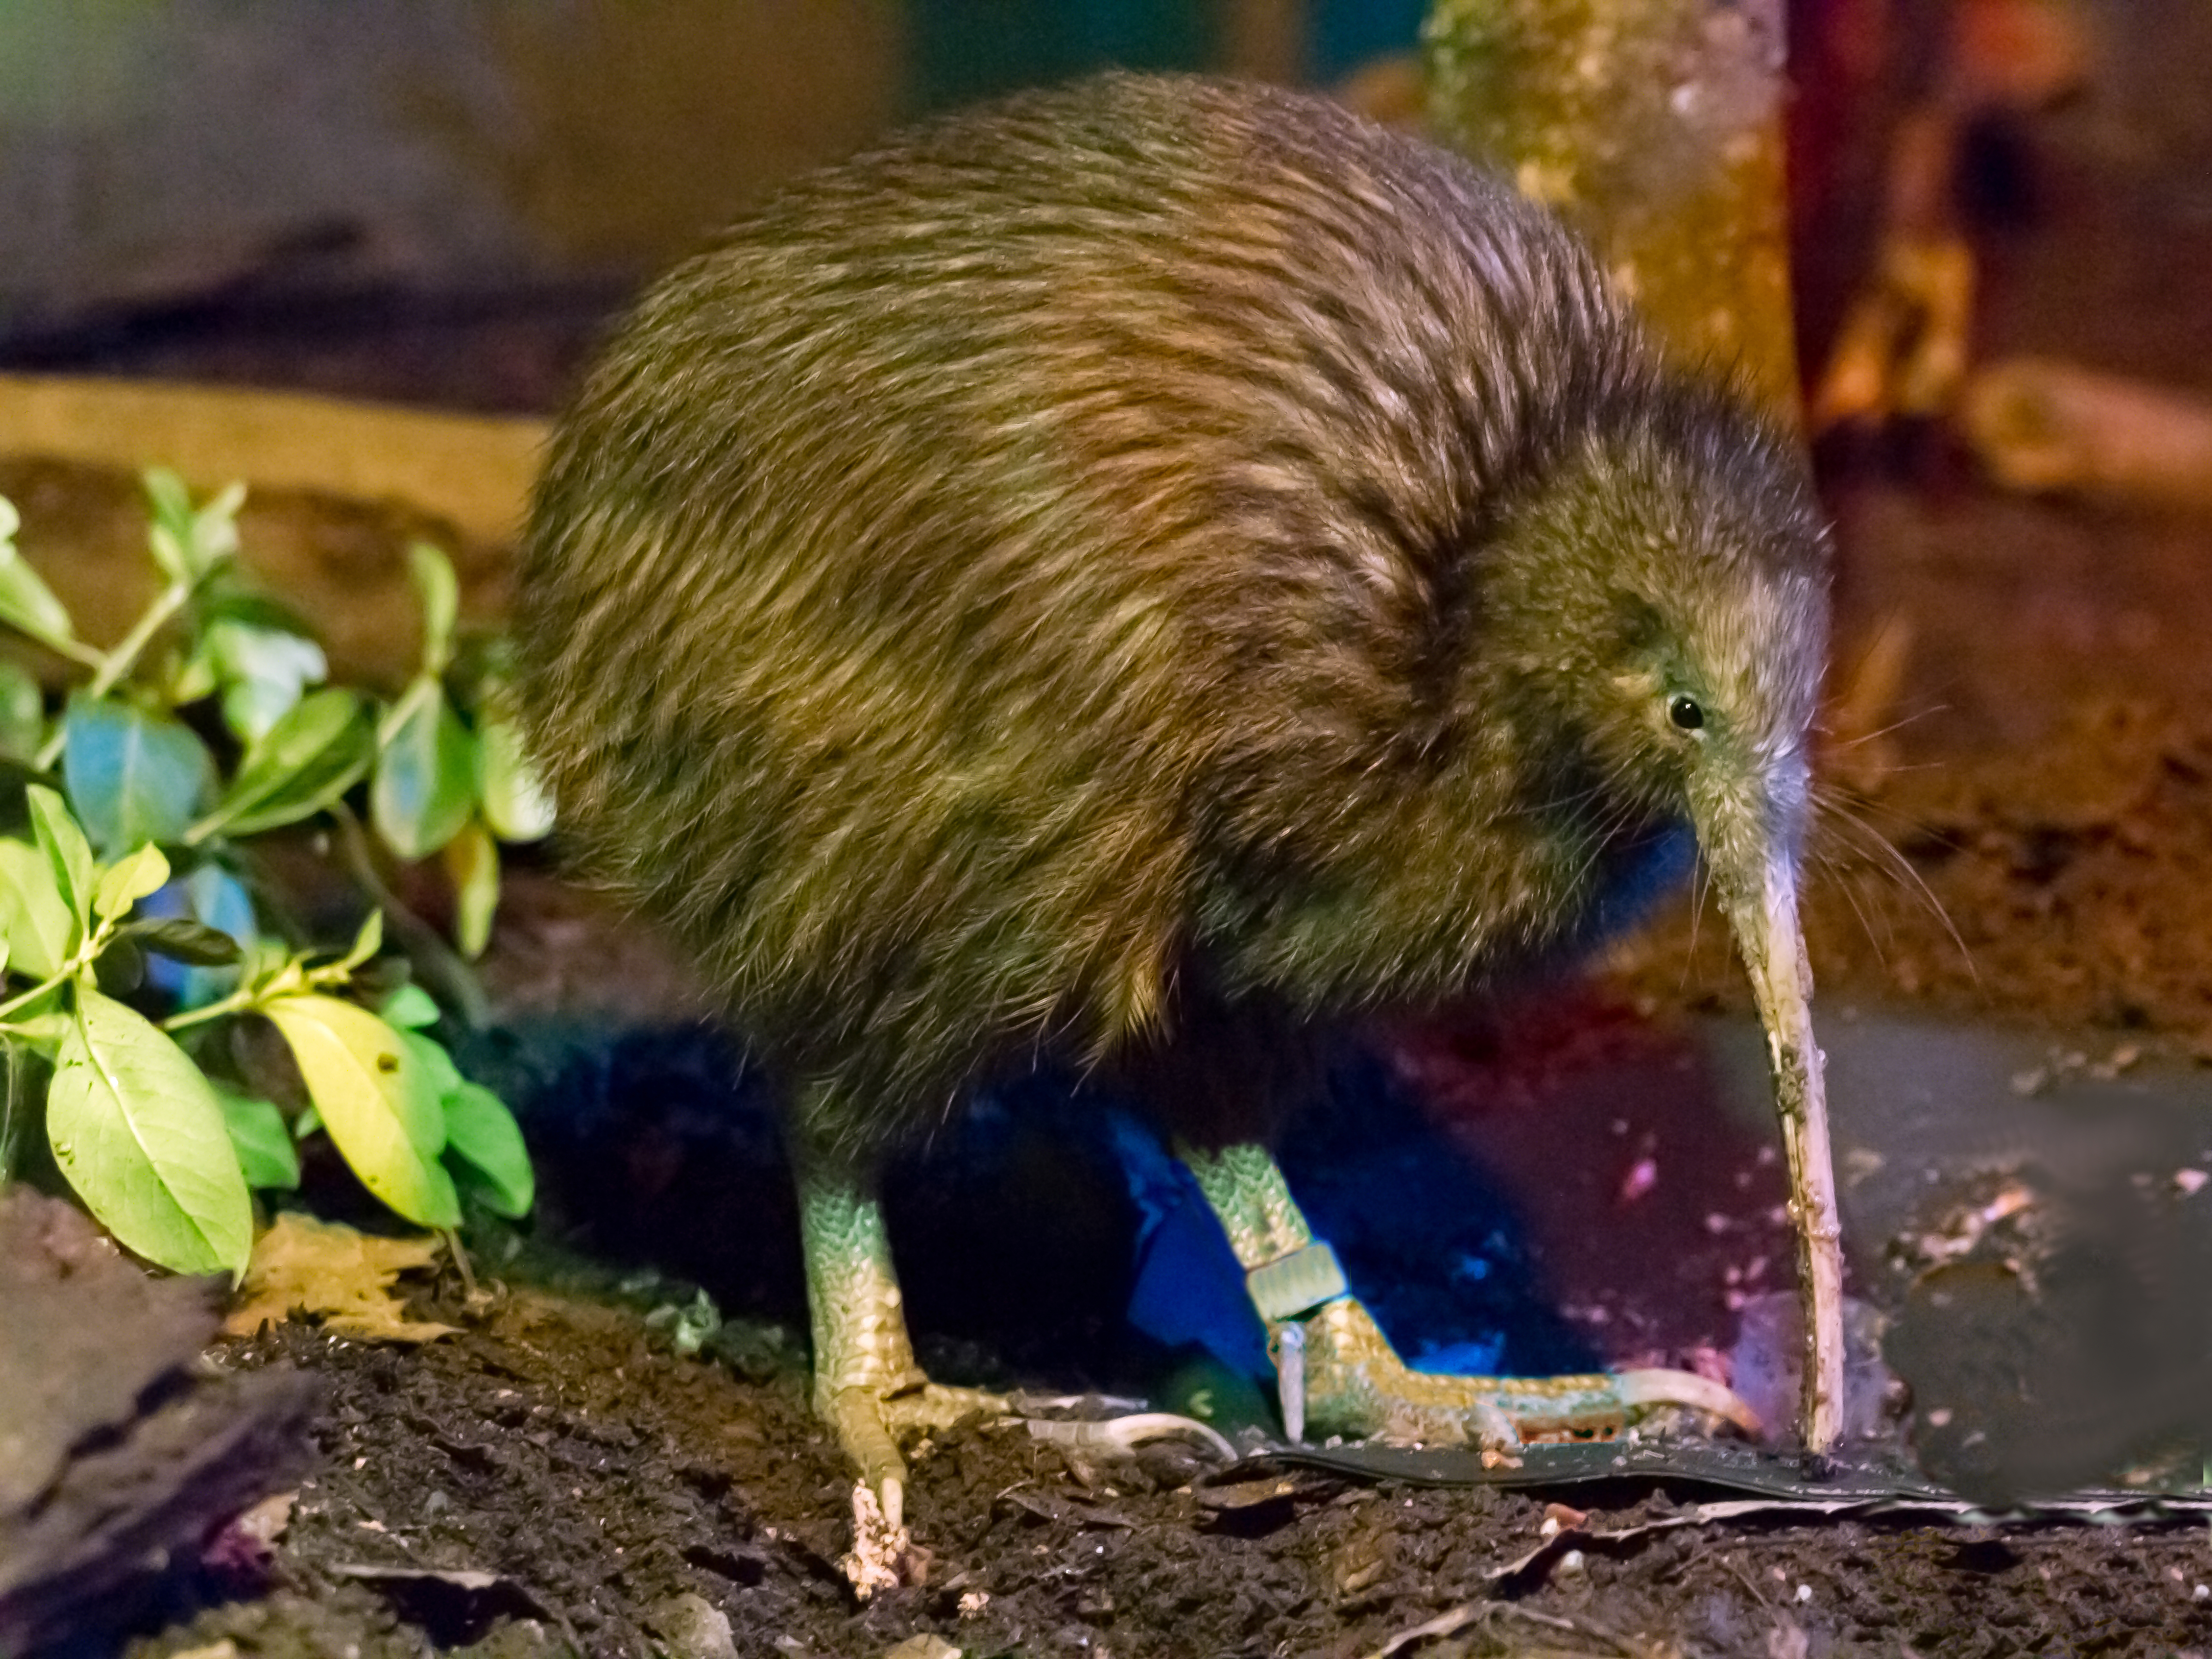
\includegraphics[width=0.1\textwidth]{\GRAPHPATH/kiwi}}}$
  \end{minipage}\\
  \Halbzeile
  \centering 
  \grau{\tiny Bildquelle: Wikipedia}
\end{frame}

\begin{frame}
  {Programmatisches Schlussbild | Antwort}
  \onslide<+->
  \onslide<+->
  Die ewige Schwachsinnsfrage: Sind Kiwis und Pinguine nun \gruen{Vögel} oder nicht?\\
  \Viertelzeile
  \grau{Nur getoppt von: Erdbeeren sind gar keine Beeren, sondern Sammelnussfrüchte.}\\
  \Zeile
  \begin{itemize}[<+->]
    \item \alert{Kognition} | \orongsch{intrinsisch nicht diskret}, sondern ähnlichkeitsbasiert und \orongsch{parallel}
      \begin{itemize}[<+->]
        \item \orongsch{Netzwerkarchitektur}
      \end{itemize}
      \Halbzeile
    \item \alert{Symbole} = Phone, Morphe, Wörter, Phrasen, \ldots | \orongsch{intrinsisch} diskret und \orongsch{linear}
      \begin{itemize}[<+->]
        \item \orongsch{akustisches} Medium | Sagen Sie mal zwei Wörter gleichzeitig!
        \item \orongsch{schriftliches} Medium | Lesen Sie mal \textit{Zettels Traum} von Arno Schmidt\\
          \grau{(inkl.\ der Versuche, mehrere Wörter "`in einem"' zu schreiben)}
      \end{itemize}
    \Halbzeile
    \item[\ding{222}] Da wir nur akustisch oder über schriftliche Artefakte kommunizieren können,\\
      \alert{muss das Sprachsystem symbolisch sein}.
    \item[\ding{222}] Da es architekturbedingt nur nicht-symbolisch verarbeiten kann,\\
      \alert{muss das Gehirn symbolische Systeme so gut wie nötig und möglich emulieren}.
  \end{itemize}
\end{frame}


\begin{frame}
  {Programmatisches Schlussbild | Ausführung}
  \onslide<+->
  \onslide<+->
  Auch nicht-verschriftete Sprache muss medial bedingt logische Eigenschaften haben.\\
  \onslide<+->
  Kulturell bilden sich stärker symbolische Modi aus, vor allem durch Schrift.\\
  \grau{\footnotesize Norm, Selbst- und Fremdkorrektur, Textplanung, intensionale Definitionen, Explizierung, \ldots}\\
  \grau{\footnotesize Warum wird das vor allem im Kontext von Schule, Fremdsprache und Bildungssprache diskutiert?}\\
  \onslide<+->
  \Zeile
  \Halbzeile
  \centering 
  \begin{tabular}[h]{cc}
    \grau{(= spontane Sprachproduktion)} & \\
    \orongsch{weniger symbolische Eigenschaften} & \small \orongsch{informelle Alltagssprache} \\
    \onslide<+->
    \textcolor{orgrA}{\faArrowDown} &\large \textcolor{orgrA}{formelle Alltagssprache} \\
    \onslide<+->
    \textcolor{orgrB}{\faArrowDown} &\Large \textcolor{orgrB}{Bildungssprache} \\
    \onslide<+->
    \textcolor{orgrC}{\faArrowDown} &\LARGE \textcolor{orgrC}{Wissenschaftssprache} \\
    \onslide<+->
    \textcolor{orgrD}{\faArrowDown} &\huge \textcolor{orgrD}{Orthosprache} \\
    \onslide<+->
    \gruen{mehr symbolische Eigenschaften} & \gruen{\Huge formales System} \\
    \grau{(= reflektierte Sprachproduktion)}  & \\
  \end{tabular}
\end{frame}

\ifdefined\HANDOUT
  \begin{frame}
    {Und was ist denn nun mit Kiwis und Pinguinen?}
    \onslide<+->
    \onslide<+->
    Unser Verständnis der Welt führt zu genaueren und diskreten Kategorisierungen,\\
    \orongsch{wo dies nötig ist}. \alert{Die Sprache folgt dem erforderlichen Maß an Genauigkeit\slash Diskretheit.}\\
    \Zeile
    \onslide<+->
    \centering
    \begin{tikzpicture}
      \node at (0cm, 0cm) {\includegraphics[height=0.6\textheight]{\GRAPHPATH/birds50}};
      \node at (5cm, 1.5cm) {\includegraphics[height=0.25\textheight]{\GRAPHPATH/kiwis}};
      \node at (5cm, -1.5cm) {\includegraphics[height=0.25\textheight]{\GRAPHPATH/penguins}};
      \path (-0.3cm, 2.5cm) edge [-latex] (4.6cm, 1.25cm);
      \path (1.1cm, -0.45cm) edge [-latex] (4.2cm, -1.725cm);
    \end{tikzpicture}\\
    \Halbzeile
    \grau{\tiny Bildquelle: Wikipedia}
  \end{frame}
\else
  \begin{frame}
    {Und was ist denn nun mit Kiwis und Pinguinen?}
    \onslide<+->
    \onslide<+->
    Unser Verständnis der Welt führt zu genaueren und diskreten Kategorisierungen,\\
    wo dies nötig ist. \alert{Die Sprache folgt diesem Maß an Genauigkeit und Diskretheit!}\\
    \Zeile
    \onslide<+->
    \centering
    \begin{minipage}{0.9\textwidth}
    \centering
      $\vcenter{\hbox{\includegraphics[height=0.7\textheight]{\GRAPHPATH/birds50}}}$\hspace{0.1\textwidth}
        \only<3>{$\vcenter{\hbox{\rule{0.4\textwidth}{0em}}}$}%
        \only<4>{$\vcenter{\hbox{\includegraphics[width=0.4\textwidth]{\GRAPHPATH/kiwis}}}$}%
        \only<5>{$\vcenter{\hbox{\includegraphics[width=0.4\textwidth]{\GRAPHPATH/penguins}}}$}
    \end{minipage}\\
    \grau{\tiny Bildquelle: Wikipedia}
  \end{frame}
\fi


\section{Linguistische Theorien}

\begin{frame}
  {"`Semantik"' im generativen T-Modell}
  \onslide<+->
  \onslide<+->
  \centering 
  \resizebox{0.6\textwidth}{!}{
    \begin{tikzpicture}

      \node [rectangle, draw, align=left, color=teal, rounded corners=0.5em] (Numeration) at (5cm, -6cm) {Numeration};
      
      \node [visible on=<3->, rectangle, draw, align=left, color=gray] (Lexikon) at (1cm, -6cm) {Lexikon};
      \path (Lexikon.east) edge [visible on=<3->, line width=0.5mm, dashed] node [below, shift={(-0.4cm,0)}] {\textit{}} (Numeration.west);
     
      \node [visible on=<4->, rectangle, draw, align=left, color=gray] (Intention) at (9cm, -6cm) {Intention};
      \path (Intention.west) edge [visible on=<4->, line width=0.5mm, dashed] node [below, shift={(-0.4cm,0)}] {\textit{}} (Numeration.east);

      \node [visible on=<5->, rectangle, draw, align=left, fill=black, color=black, rounded corners=0.5em] (Syntax) at (5cm, -4.5cm) {\whyte{Syntax}};
      \path (Numeration.north) edge [visible on=<5->, line width=0.5mm, -latex] node [below, shift={(-0.4cm,0)}] {\textit{}} (Syntax.south);  

      \node [visible on=<6->, rectangle, draw, align=left, color=teal, rounded corners=0.5em] (Phrasenstruktur) at (5cm, -3cm) {Phrasenstruktur};
      \path (Syntax.north) edge [visible on=<6->, line width=0.5mm, -latex] node [below, shift={(-0.4cm,0)}] {\textit{}} (Phrasenstruktur.south);  

      \node [visible on=<7->, rectangle, draw, align=left, color=teal, rounded corners=0.5em] (PF) at (4cm, 0cm) {PF};
      \path (Phrasenstruktur.north) edge [visible on=<7->, line width=0.5mm, -latex] node [below, shift={(-0.4cm,0)}] {\textit{}} (PF.south);  
     
      \node [visible on=<8->, rectangle, draw, align=left, color=gray] (Aeusserung) at (1cm, 0cm) {Äußerung};
      \path (Aeusserung.east) edge [visible on=<8->, line width=0.5mm, dashed] node [below, shift={(-0.4cm,0)}] {\textit{}} (PF.west);
     
      \node [visible on=<9->, rectangle, draw, align=left, fill=black, color=black, rounded corners=0.5em] (Syntax2) at (6cm, -1.5cm) {\whyte{Syntax 2}};
      \path (Phrasenstruktur.north) edge [visible on=<9->, line width=0.5mm, -latex] node [below, shift={(-0.4cm,0)}] {\textit{}} (Syntax2.south);  
     
      \node [visible on=<10->, rectangle, draw, align=left, color=teal, rounded corners=0.5em] (LF) at (6cm, 0cm) {LF};
      \path (Syntax2.north) edge [visible on=<10->, line width=0.5mm, -latex] node [below, shift={(-0.4cm,0)}] {\textit{}} (LF.south);  

      \node [visible on=<11->, rectangle, draw, align=left, color=gray] (Interpretation) at (9cm, 0cm) {Interpretation};
      \path (Interpretation.west) edge [visible on=<11->, line width=0.5mm, dashed] node [below, shift={(-0.4cm,0)}] {\textit{}} (LF.east);
      
    \end{tikzpicture}
  }
\end{frame}

\begin{frame}
  {Repräsentationsebenen}
  \onslide<+->
  \onslide<+->
  Im klassischen generativen Modell:\\
  \grau{\footnotesize (In minimalistischen Modellen herrscht -- Chomsky muss es mögen! -- sowieso Anarchie.)}
  \Zeile
  \begin{itemize}[<+->]
    \item keine echte Interpretation auf LF
    \item Bewegung \rot{nachdem} der Satz geäußert wurde
    \item Herstellung einer logisch interpretierbaren \alert{Form} auf LF
    \item Grund | Syntax kann nicht alle Interpretationen abbilden
      \Halbzeile
      \begin{itemize}[<+->]
        \item[ ] \alert{Klassiker Quantorenskopus}
        \item[ ] \textit{Everybody loves somebody.}
          \Viertelzeile
        \item[A] Für alle Personen y gilt, dass es eine Person x gibt, für die gilt: y liebt x \grau{| $(\forall y)(\exists x)L(y,x)$}
        \item[B] Es gibt eine Person x, sodass für alle Personen y gilt: y liebt x \grau{| ($\exists x)(\forall y)L(y,x)$}
      \end{itemize}
  \end{itemize}
\end{frame}


\begin{frame}
  {Montagues direkte Interpretation}
  \onslide<+->
  \onslide<+->
  Sprache ist Logik ist Sprache \ldots\\
  \Halbzeile
  \begin{itemize}[<+->]
    \item[A] Entweder ist die \alert{Übersetzung in eine LF trivial und äquivalent zur PF\slash Syntax},\\
      oder \orongsch{sie fügt etwas hinzu, das der Sprache an sich fehlt}.
    \item[B] Sätze haben aber auch \alert{mit LF-Übersetzung nur die Bedeutungen,\\
      die sie sowieso haben} \grau{(keine Hinzufügung)}.
    \item[\ding{222}] Also ist die \gruen{Übersetzung in LF trivial und äquivalent zur PF\slash Syntax}.
    \item[\ding{222}] Wir können \gruen{Sätze direkt interpretieren} (wie sie gesprochen\slash geschrieben werden).
     \Zeile 
   \item \alert{Montagues \textit{lf}} | direkte Übersetzung von sprachlichen in logische Ausdrücke
  \end{itemize}
\end{frame}

\section{Referentielle Semantik basal}

\begin{frame}
  {Interessante Eigenschaften von Sprache}
  \onslide<+->
  \begin{itemize}[<+->]
    \item Aussagen über die\slash Teile der Welt
    \item Ausdrücke bezeichnen\slash referieren auf Dinge i.\,w.\,S.
    \item Informativität
    \item objektiv beurteilbar (\zB Wahrheit von Sätzen)
      \Zeile
    \item \alert{Aber welche sprachlichen Einheiten referieren auf was?}
  \end{itemize}
\end{frame}

\begin{frame}
  {Referenz | Eigennamen}
  \onslide<+->
  \onslide<+->
  Ein \alert{Eigenname} \ding{222} \alert{genau ein Objekt} in der Welt\\
  \onslide<+->
  \Zeile
  \centering
    \begin{tikzpicture}
      \node [] (name) at (-6cm, 0cm) {\textit{Jan Böhmermann}};
      \node [visible on=<4->] (boehmi) at (0cm, 0cm) {
\includegraphics[width=0.2\textwidth]{\GRAPHPATH/boehmermann}};
      \path (name.east) edge [visible on=<4->, line width=0.5mm, -latex] node {\textit{}} (boehmi.west);
    \end{tikzpicture}
\end{frame}

\begin{frame}
  {Referenz | Appellativa}
  \onslide<+->
  \onslide<+->
  Ein normales \alert{Nomen} \ding{222} \alert{eine Menge von Objekten} in der Welt\\
  \onslide<+->
  \Zeile
  \centering
    \begin{tikzpicture}
      \node [] (noun) at (-6cm, 0cm) {\textit{soldier}};
      \node [visible on=<4->] (soldiers) at (0cm, 0cm) {\includegraphics[width=0.2\textwidth]{\GRAPHPATH/soldiers}};
      \path (noun.east) edge [visible on=<4->, line width=0.5mm, -latex] node {\textit{}} (soldiers.west);
    \end{tikzpicture}
\end{frame}

\begin{frame}
  {Referenz | Adjektive und Verben}
  \onslide<+->
  \onslide<+->
  Ein (intersektives) \alert{Adjektiv} oder ein \alert{Verb} \ding{222} \alert{eine Menge von Objekten} in der Welt\\
  \onslide<+->
  \Zeile
  \centering
    \begin{tikzpicture}
      \node [] (adj) at (-6cm, 0cm) {\textit{human}};
      \node [visible on=<4->] (boehmi) at (0cm, +2cm) {
\includegraphics[width=0.1\textwidth]{\GRAPHPATH/boehmermann}};
      \path (adj.east) edge [visible on=<4->, line width=0.5mm, -latex] node {\textit{}} (boehmi.west);
      \node [visible on=<5->] (soldiers) at (0cm, 0cm) {\includegraphics[width=0.1\textwidth]{\GRAPHPATH/soldiers}};
      \path (adj.east) edge [visible on=<5->, line width=0.5mm, -latex] node {\textit{}} (soldiers.west);
      \node [visible on=<6->] (crowd) at (0cm, -2cm) {\includegraphics[width=0.1\textwidth]{\GRAPHPATH/crowd}};
      \path (adj.east) edge [visible on=<6->, line width=0.5mm, -latex] node {\textit{}} (crowd.west);
    \end{tikzpicture}
\end{frame}

\begin{frame}
  {Referenz | Sätze}
  \onslide<+->
  \onslide<+->
  Ein \alert{Satz} \ding{222} in erster Näherung \alert{ein Sachverhalt}\\
  \onslide<+->
  \Zeile
  \centering
    \begin{tikzpicture}
      \node [align=left] (s) at (-6cm, 0cm) {\it A humming bird\\\it is hovering over\\\it a red flower.};

      \node [visible on=<4->, align=center] (hum) at (0cm, +2cm) {\includegraphics[width=0.2\textwidth]{\GRAPHPATH/hummingbird}};
      \path (s.east) edge [visible on=<4->, line width=0.5mm, -latex] node {\textit{}} (hum.west);
      
      \node [visible on=<5->, align=center] (boehmi) at (0cm, -2cm) {
\includegraphics[width=0.2\textwidth]{\GRAPHPATH/boehmermann}\\\footnotesize (als Individuum)};
      \path (s.east) edge [visible on=<5->, line width=0.5mm, -latex, color=red] node {\textit{}} (boehmi.west);
      \node [visible on=<6->, align=center, color=red, fill=red] (nein) at (-3.5cm, -1.25cm) {\footnotesize \whyte{Nein! falsche}\\\footnotesize \whyte{Art von Objekt}};
    \end{tikzpicture}
\end{frame}

\begin{frame}
  {Freges Prinzip | Das hier wollen wir formalisieren!}
  \onslide<+->
  \onslide<+->
  Bedeutung ist kompositional!\\
  \Halbzeile
  \begin{itemize}[<+->]\small
    \item \textit{humming bird} \ding{222} die \alert{Menge} der Kolibri-Objekte
    \item \textit{a} \ding{222} \alert{Existenzaussage} für ein Element aus einer Menge
    \item \textit{a humming bird} \ding{222} \alert{Existenzaussage} für ein Element $x$\\
      aus der Menge der Kolibri-Objekte
    \item \textit{is hovering} \ding{222} die \alert{Menge} der schwebenden Objekte
    \item \textit{a humming bird is hovering} \ding{222} das existierende Kolibri-Objekt $x$\\
      ist auch ein \alert{Element der Menge} der schwebenden Objekte
    \item \textit{a red flower} \ding{222} \alert{Existenzaussage} für ein Element $y$\\
      aus der \alert{Schnittmenge} der roten Objekte und der Blumen-Objekte
    \item \textit{over} \ding{222} die \alert{Relation} zwischen Objekten (s.\ nächste Woche),\\
      die sich übereinander befinden
    \item \textit{A Humming is hovering over a red flower.} \ding{222}\\
      \gruen{Es gibt ein Objekt $x$ aus der Schnittmenge der Kolibri- und der schwebenden Objekte,\\
      und es gibt ein Objekt $y$ aus der Schnittmenge der roten und der Blumen-Objekte,\\
    und $x$ befindet sich über $y$.}
  \end{itemize}
\end{frame}

\section{Semantische Eigenschaften von Sätzen}

\begin{frame}
  {Implikation (Entailment)}
  \onslide<+->
  \onslide<+->
  Mengen von Aussagesätzen \alert{implizieren} andere Sätze.\\
  \onslide<+->
  Sätze (Implikationen) lassen sich aus anderen Sätzen (Axiome) \alert{beweisen}.\\
  \Halbzeile
  \begin{itemize}[<+->]
    \item[A] \textit{Jan Böhmermann ist ein Mensch.}
    \item[B] \textit{Jan Böhmermann ist leutselig.}
    \item[C] \textit{Jan Böhmermann ist ein leutseliger Mensch.}
      \Halbzeile
    \item[ ] \alert{$A,B\vdash C$} | A und B implizieren C. (C ist beweisbar aus A und B.)
    \item[ ] \rot{$A\not\vdash C$} | A impliziert nicht C.
    \item[ ] \rot{$B\not\vdash C$} | B impliziert nicht C.
      \Halbzeile
    \item[ ] \orongsch{$A\vdash A\wedge A$} \onslide<+->| \textit{Jan Böhmermann ist ein Mensch \orongsch{und} Jan Böhmermann ist ein Mensch.}
      \Halbzeile
    \item[D] \textit{Irgendetwas ist ein Mensch.}
    \item[ ] \alert{$A\vdash D$} 
  \end{itemize}
\end{frame}

\begin{frame}
  {Tests auf Implikation}
  \onslide<+->
  \onslide<+->
  Wenn diese Kriterien zutreffen, impliziert A B:\\
  \Zeile
  \begin{itemize}[<+->]
    \item Wenn A wahr ist, ist B auch immer wahr.
    \item Eine Situation, die von B beschrieben wird, wird auch von A beschrieben.
    \item Die Information in B ist vollständig in der Information in A enthalten.
    \item Man kann unter keinen Umständen sagen: \textit{A ist wahr, aber B ist nicht wahr.}
  \end{itemize}
\end{frame}

\begin{frame}
  {Übung | Sind das Implikationen?}
  \begin{itemize}[<+->]\small
    \item Böhmermann ist Showmaster. $\vdash$ Böhmermann ist menschlich.
    \item Böhmermann ist nicht sehr groß. $\vdash$ Irgendjemand ist nicht sehr groß.
    \item Böhmermann ist nicht sehr groß. $\vdash$ Irgendjemand ist sehr groß.
    \item Manche Menschen sind leutselig. $\vdash$ Böhmermann ist leutselig.
    \item Ich habe das neue drip-133-Album gehört. $\vdash$ drip-133 hat ein neues Album veröffentlicht.
    \item Nachdem ich einen Sherry getrunken habe, habe ich den Kondensator getauscht.\\
      $\vdash$ Ich habe einen Sherry getrunken.
    \item Nachdem Linux nicht mehr startete, habe ich einen weiteren Sherry getrunken.\\
      $\vdash$ Linux ist noch nie gestartet.
    \item Mein ehemaliger Mitbewohner mag Becks.\\
      $\vdash$ Mein ehemaliger Mitbewohner könnte Sherry mögen.
    \item Böhmermann hat das heutige ZDF Magazin beendet.\\
      $\vdash$ Das heutige ZDF Magazin wurde beendet.
  \end{itemize}
\end{frame}

\begin{frame}
  {Synonymie}
  \onslide<+->
  \onslide<+->
  Synonyme Ausdrücke haben \orongsch{exakt} \alert{die gleiche Referenz}.\\
  \Halbzeile
  \begin{itemize}[<+->]
    \item lexikalische Synonymie | \textit{humming bird} $\stackrel{lex}{\equiv}$ \textit{colibri}
      \Halbzeile
    \item kompositionale Synonymie
      \begin{itemize}[<+->]
        \item[ ] \textit{Mulder traf seine entführte Schwester, nachdem er\\
          in die geheime Militärbasis eingebrochen war.}
        \item[$\equiv$] \textit{Bevor er seine entführte Schwester traf,\\
          brach Mulder in die geheime Militärbasis ein.}
      \end{itemize}
    \Halbzeile
    \item \alert{$A\equiv B\ \text{gdw}\ A\vdash B\ \text{und}\ B\vdash A$} (gegenseitige Implikation)
    \item \grau{\textit{gdw} = \textit{genau dann wenn} | \textit{iff} = \textit{if and only if}}
  \end{itemize}
\end{frame}

\section{Referenz von Sätzen}

\begin{frame}
  {Natürliche Sprache und Implikation}
  \onslide<+->
  \onslide<+->
  Referentielle Semantik \orongsch{modelliert mehr als} \alert{einfaches Zeigen auf Objekte durch Sprache}.\\
  \Viertelzeile
  \onslide<+->
  Zusätzliche Logik für Fälle wie diesen (und viele andere):\\
  \Zeile
  \onslide<+->
  \begin{tabular}[h]{lll}
    & \alert{\textit{Die Lieblingsblume meines Kolibris}} & \textit{ist rot.} \\
    \visible<6->{\orongsch{$\vdash$}} & \visible<5->{\alert{\textit{Eine Blume}} & \textit{ist rot.}} \\
  \end{tabular}
\end{frame}

\begin{frame}
  {Synonyme NPs}
  \onslide<+->
  \begin{itemize}[<+->]
    \item[a] \textit{colibri}
    \item[b] \textit{humming bird}
    \item[ ] \gruen{$a\stackrel{lex}{\equiv} b$}
      \Halbzeile
    \item[c] \textit{a brunette lady}
    \item[d] \textit{a brown-haired dame}
    \item[ ] \gruen{$c\equiv d$}
      \Halbzeile
    \item[e] \textit{the primates}
    \item[f] \textit{the apes and humans}
    \item[ ] \gruen{$e\equiv f$}
  \end{itemize}
\end{frame}

\begin{frame}
  {Ausgelassen: The Slingshot Argument}
  \onslide<+->
  \onslide<+->
  Das \textit{Slingshot Argument}:
  \begin{itemize}[<+->]
    \item Alle wahren Sätze haben dieselbe Bedeutung (1).
    \item Alle falschen Sätze haben dieselbe Bedeutung (0).
    \item Diese Bedeutung ist ihr \alert{Wahrheitswert}.
    \item In ausformulierten Semantiken ist das ihr \alert{Extension}.
    \item Die mehr ``inhaltliche'' Bedeutung eines Satzes\\
      wird dann als seine \alert{Intension} modelliert.
  \end{itemize}
  \Halbzeile
  \centering 
  \onslide<+->
  \grau{\scriptsize Der Beweis ist komplexer, s.\ \citet{Church1948}.\\
    Etwas zugänglicher in \url{https://plato.stanford.edu/entries/truth-values/slingshot-argument.html}}
\end{frame}

\begin{frame}
  {Synonymie von Konstituenten und Sätzen}
  Synonymie von Konstituenten im Satzkontext \ding{222} Satzsynonymie\\
  \onslide<+->
  \Halbzeile
  \begin{itemize}[<+->]
    \item[A] \alert{\textit{A \orongsch{colibri} is hovering over a red flower.}}
    \item[B] \alert{\textit{A \orongsch{humming bird} is hovering over a red flower.}}
    \item[ ] \gruen{$A\equiv B$ weil $a\equiv b$ und Satzkontext identisch}
    \item[ ] \gruen{$[\Sub{A} a]\equiv[\Sub{B} b]$ wenn $a\equiv b$ und $[\Sub{A} \_]=[\Sub{B} \_]$}
      \Halbzeile
    \item[C] \alert{\textit{Lauren Bacall was \orongsch{a brunette lady}.}}
    \item[D] \alert{\textit{Lauren Bacall was \orongsch{a brown-haired dame}.}}
    \item[ ] \gruen{$C\equiv D$ weil $c\equiv d$ und Satzkontext identisch}
      \Halbzeile
    \item[E] \alert{\textit{\orongsch{Primates} are intelligent.}}
    \item[F] \alert{\textit{\orongsch{The apes and humans} are intelligent.}}
    \item[ ] \gruen{$E\equiv F$ weil $e\equiv f$ und Satzkontext identisch}
  \end{itemize}
\end{frame}

\section{Reden in Fragmenten}

\begin{frame}
  {Grammatik- und Semantikfragmente}
  \onslide<+->
  \onslide<+->
  \alert{Konstruktive}, \alert{schrittweise} Annäherungen an sprachliche Modellierung\\
  \Zeile
  \begin{itemize}[<+->]
    \item Grammatikfragment | Ausschnitt einer Gesamtgrammatik
    \item erwünschte schrittweise Erweiterung von Fragmenten (vgl.\ HPSG)
      \Zeile
    \item Konstruktion eines Semantik-Fragments
      \begin{itemize}[<+->]
         \item grammatische Kategorien und Referenzen von Wörtern
         \item Grammatikmechanismen und zugehörige Bedeutungskonstruktion
         \item Ergebnis | Semantik von Sätzen und Beitrag aller Konstituenten dazu
      \end{itemize}
    \item \Halbzeile
      \alert{T-Sätze}
      \begin{itemize}[<+->]
        \item \alert{L} eine Sprache, \alert{S} ein Satz, \alert{v} ein Sachverhalt, \alert{p} eine Aussage über Wahrheitsbedingungen
        \item \alert{S aus L ist wahr in v gdw p.}
      \end{itemize}
  \end{itemize}
\end{frame}

\begin{frame}
  {Das Lexikon}
  \onslide<+->
  \onslide<+->
  Die folgenden simplexen Ausdrücke sind Teil von F\Sub{1}.\\
  \onslide<+->
  Kein anderer simplexer Ausdruck ist Teil von F\Sub{1}.\\
  \Halbzeile
  \begin{enumerate}[<+->]
    \item N $\rightarrow$ \emph{Herr Webelhuth, Frau Klenk, the Turm-Mensa} \label{lex01}
    \item V\Sub{{i}} $\rightarrow$ \emph{is relaxed, is creative, is stupid} \label{lex02}
    \item V\Sub{t} $\rightarrow$ \emph{prefers} \label{lex03}
    \item conj $\rightarrow$ \emph{and, or} \label{lex04}
    \item neg $\rightarrow$ \emph{it is not the case that} \label{lex05}
  \end{enumerate}
\end{frame}

\begin{frame}
  {Die Phrasenstrukturgrammatik von F\Sub{1}}
  \onslide<+->
  \onslide<+->
  Folgende Kompositionsregeln sind Teil von F\Sub{1}.\\
  Keine andere Kompositionsregel ist Teil von F\Sub{1}.\\
  \Halbzeile
  \begin{enumerate}[<+->]
    \item S $\rightarrow$ N VP \label{syn01}
    \item S $\rightarrow$ S conj S \label{syn02}
    \item S $\rightarrow$ neg S \label{syn03}
    \item VP $\rightarrow$ V\Sub{{i}} \label{syn04}
    \item VP $\rightarrow$ V\Sub{t} N \label{syn05}
  \end{enumerate}
\end{frame}

\begin{frame}
  {Referenz simplexer Ausdrücke}
  \begin{itemize}[<+->]
    \item $\llbracket$Herr Webelhuth$\rrbracket$ = Herr Webelhuth \label{lexint01}
    \item $\llbracket$Frau Klenk$\rrbracket$ = Frau Klenk \label{lexint02}
    \item $\llbracket$the Turm-Mensa$\rrbracket$ = the Turm-Mensa \label{lexint03}
    \item $\llbracket$is relaxed$\rrbracket$ = $\{x:x\ is\ relaxed\}$ \label{lexint04}
    \item $\llbracket$is creative$\rrbracket$ = $\{x:x\ is\ creative\}$ \label{lexint05}
    \item $\llbracket$is stupid$\rrbracket$ = $\{x:x\ is\ stupid\}$ \label{lexint06}
    \item $\llbracket$prefers$\rrbracket$ = $\{\langle x,y\rangle: x\ prefers\ y\}$ \label{lexint07}
  \end{itemize}
\end{frame}

\begin{frame}
  {Referenz von Funktionswörtern}
  Funktionswörter referieren auf \alert{Funktionen}.\\
  \Zeile
  \begin{itemize}[<+->]
    \item $\dem{neg} = \left[
                       \begin{array}{l}
                                1 \rightarrow 0\\
                                0 \rightarrow 1
                       \end{array}
                     \right]$ \label{fint01}
    \item $\dem{and} = \left[
                       \begin{array}{l}
                                \langle 1,1 \rangle \rightarrow 1\\
                                \langle 1,0 \rangle \rightarrow 0\\
                                \langle 0,1 \rangle \rightarrow 0\\
                                \langle 0,0 \rangle \rightarrow 0
                       \end{array}
                       \right]$ \label{fint02}
    \item $\dem{or} = \left[
                           \begin{array}{l}
                                    \langle 1,1 \rangle \rightarrow 1\\
                                    \langle 1,0 \rangle \rightarrow 1\\
                                    \langle 0,1 \rangle \rightarrow 1\\
                                    \langle 0,0 \rangle \rightarrow 0
                           \end{array}
                           \right]$ \label{fint03}
  \end{itemize}
\end{frame}

\begin{frame}
  {T-Sätze für F\Sub{1}}
  \begin{itemize}[<+->]
    \item \den{\alert{[\Sub{S}{ }N{ }VP]}} = 1 iff $\den{N}\in\den{VP}$, else $0$ \label{t01}
    \item \den{\alert{[\Sub{S} S1 conj S2]}} = $\den{conj}(\langle\den{S1},\den{S2}\rangle)$ \label{t02}
    \item \den{\alert{[\Sub{S} neg S]}} = $\den{neg}(\den{S})$ \label{t03}
    \item \den{\alert{[\Sub{VP} V\Sub{t} N]}} = $\{x:\langle x,\den{N}\rangle\in\den{V\Sub{t}}\}$ \label{t04}
      \Halbzeile
    \item für einen nicht verzweigenden Knoten K und seine Tochter D: $\dem{[\Sub{K} D]}=\dem{D}$ \label{t05}
      \Halbzeile
    \item \grau{Das geht alles eleganter. Bitte etwas Geduld!}
  \end{itemize}
\end{frame}

\begin{frame}
  {Schritt 1 | Syntax parsen}
  Ist folgendes ein Satz aus F\Sub{1}? \onslide<+-> \alert{\textit{Herr Webelhuth is relaxed.}}\\
  \Halbzeile
  \begin{itemize}[<+->]
    \item{} [\Sub{N} \textit{Herr Webelhuth}] mit \gruen{Lexikonregel \ref{lex01}}
    \item{} [\Sub{V\Sub{i}} \textit{is relaxed}] mit \gruen{Lexikonregel \ref{lex02}}
    \item{} [\Sub{VP} [\Sub{V\Sub{i}} \textit{is relaxed}]] mit \gruen{Syntaxregel \ref{syn04}}
    \item{} [\Sub{S} [\Sub{N} \textit{Herr Webelhuth}] \Sub{VP} [\Sub{V\Sub{i}} \textit{is relaxed}]] mit \gruen{Syntax \ref{syn01}}
  \end{itemize}
\end{frame}

\begin{frame}
  {Syntax als Baum}
  \centering 
  \begin{forest}
    [S
      [N
        [\textit{Herr Webelhuth}]
      ]
      [VP
        [V\Sub{i}
          [\textit{is relaxed}]
        ]
      ]
    ]
  \end{forest}
\end{frame}

\begin{frame}
  {Semantik | Referenz der Teile und ihrer Bedeutung}
  \onslide<+->
  \onslide<+->
  \alert{v} (Sachverhalt) | Herr Webelhuth (das ontologische Objekt) $\in\{x: x\ is\ relaxed\}$\\
  \Halbzeile
  \begin{itemize}[<+->]
    \item für N: \den{\textit{Herr Webelhuth}} = Herr Webelhuth (das ontologische Objekt)
    \item für VP (und V\Sub{i}): \den{\textit{is relaxed}} = $\{x:x\ is\ relaxed\}$ (enthält Herrn Webelhuth)
    \item für S: \den{[\Sub{S}{ }N{ }VP]} = 1 iff \den{N} $\in$ \den{VP}, else 0
      \Halbzeile
    \item in v daher \gruen{\den{[\Sub{S} \textit{Herr Webelhuth is relaxed.}]}=1}
  \end{itemize}
\end{frame}

\ifdefined\HANDOUT
  \begin{frame}
    {Semantik im Baum}
    \begin{tabular}[h]{cc}
    \onslide<+->
    \onslide<+->
    \centering 
    \begin{forest}
      [\den{S}
        [\den{N}
          [\den{\textit{Herr Webelhuth}}]
        ]
        [\den{VP}
          [\den{V\Sub{i}}
            [\den{\textit{is relaxed}}]
          ]
        ]
      ]
    \end{forest} &%
    \begin{forest}
      [\gruen{1} \alert{because Herr Webelhuth$\in$\{x:x is relaxed\}}
        [\grau{Herr Webelhuth}
          [\gruen{Herr Webelhuth}]
        ]
        [\grau{\{x:x is relaxed\}}
          [\grau{\{x:x is relaxed\}}
            [\gruen{\{x:x is relaxed\}}]
          ]
        ]
      ]
    \end{forest}
    \\
    \end{tabular}
  \end{frame}
\else
  \begin{frame}
    {Semantik im Baum}
    \begin{tabular}[h]{cc}
    \onslide<+->
    \onslide<+->
    \centering 
    \begin{forest}
      [\den{S}, whytetree
        [\den{N}
          [\den{\textit{Herr Webelhuth}}]
        ]
        [\den{VP}
          [\den{V\Sub{i}}
            [\den{\textit{is relaxed}}]
          ]
        ]
      ]
    \end{forest} &%
    \begin{forest}
      [\gruen{1} \alert{because Herr Webelhuth$\in$\{x:x is relaxed\}}
        [\grau{Herr Webelhuth}
          [\gruen{Herr Webelhuth}]
        ]
        [\grau{\{x:x is relaxed\}}
          [\grau{\{x:x is relaxed\}}
            [\gruen{\{x:x is relaxed\}}]
          ]
        ]
      ]
    \end{forest}
    \\
    \end{tabular}
  \end{frame}
\fi

\begin{frame}
  {Komplexere Phrasenstrukturen}
  \alert{[\Sub{S\Sub{1}} \textit{Frau Klenk is creative}]} \textit{and it is not the case that} \orongsch{[\Sub{S\Sub{2}} \textit{Herr Webelhuth is relaxed}]}\\
  and \gruen{[\Sub{S\Sub{3}} \textit{Frau Klenk prefers the Turm-Mensa}]}.\\
  \Halbzeile
  \centering
  \scalebox{0.8}{
    \begin{forest}
      [S
        [\alert{S\Sub{1}}, bluetree
          [N, bluetree
            [\textit{Frau Klenk}]
          ]
          [VP, bluetree
            [\textit{is creative}, narroof]
          ]
        ]
        [conj
          [\textit{and}]
        ]
        [S
          [neg
            [\textit{it is not the case that}]
          ]
          [S
            [S\Sub{2}, orongschtree
              [N, orongschtree
                [\textit{Herr Webelhuth}]
              ]
              [VP, orongschtree
                [\textit{is relaxed}, narroof]
              ]
            ]
            [conj
              [\it and]
            ]
            [S\Sub{3}, gruentree
              [N, gruentree
                [\textit{Frau Klenk}]
              ]
              [VP, gruentree
                [V\Sub{t}, gruentree
                  [\textit{prefers}]
                ]
                [N, gruentree
                  [\textit{the Turm-Mensa}]
                ]
              ]
            ]
          ]
        ]
      ]
    \end{forest}
  }
\end{frame}

\begin{frame}
  {Interpretation}
  \onslide<+->
  \onslide<+->
  Die Situation\slash die Umstände v sind:\\
  \Halbzeile
  \begin{itemize}[<+->]
    \item $\text{Herr Webelhuth}\in\{x: x\text{ is relaxed}\}$
    \item $\text{Frau Klenk}\in\{x: x\text{ is creative}\}$
    \item $\langle\text{Frau Klenk, Turm-Mensa}\rangle\not\in\{\langle x,y\rangle: x\text{ prefers }y\}$
  \end{itemize}
\end{frame}

\ifdefined\HANDOUT
  \begin{frame}
    {Die Interpretation komplexerer Phrasenstrukturen}
    \onslide<+->
    \onslide<+->
    \begin{itemize}
      \item \orongsch<13->{$\text{Herr Webelhuth}\in\{x: x\text{ is relaxed}\}$}
      \item \alert<8->{$\text{Frau Klenk}\in\{x: x\text{ is creative}\}$}
      \item \gruen<21->{$\langle\text{Frau Klenk, Turm-Mensa}\rangle\not\in\{\langle x,y\rangle: x\text{ prefers }y\}$}
    \end{itemize}
    \onslide<+->
    \Halbzeile
    \centering 
    \scalebox{0.55}{
      \begin{forest}
        [\den{S}
          [\den{S\Sub{1}}, bluetree
            [\den{N}, bluetree
              [\den{\textit{Frau Klenk}}]
            ]
            [\den{VP}, bluetree
              [\den{\textit{is creative}}, narroof]
            ]
          ]
          [\den{conj}
            [\den{\textit{and}}]
          ]
          [\den{S}
            [\den{neg}
              [\den{\textit{it is not the case that}}]
            ]
            [\den{S}
              [\den{S\Sub{2}}, orongschtree
                [\den{N}, orongschtree
                  [\den{\textit{Herr Webelhuth}}]
                ]
                [\den{VP}, orongschtree
                  [\den{\textit{is relaxed}}, narroof]
                ]
              ]
              [\den{conj}
                [\den{\it and}]
              ]
              [\den{S\Sub{3}}, gruentree
                [\den{N}, gruentree
                  [\den{\textit{Frau Klenk}}]
                ]
                [\den{VP}, gruentree
                  [\den{V\Sub{t}}, gruentree
                    [\den{\textit{prefers}}]
                  ]
                  [\den{N}, gruentree
                    [\den{\textit{the Turm-Mensa}}]
                  ]
                ]
              ]
            ]
          ]
        ]
      \end{forest}
    }
  \end{frame}

  \addtocounter{framenumber}{-1}
  \begin{frame}
    {Die Interpretation komplexerer Phrasenstrukturen}
    \onslide<+->
    \onslide<+->
    \begin{itemize}
      \item \orongsch<13->{$\text{Herr Webelhuth}\in\{x: x\text{ is relaxed}\}$}
      \item \alert<8->{$\text{Frau Klenk}\in\{x: x\text{ is creative}\}$}
      \item \gruen<21->{$\langle\text{Frau Klenk, Turm-Mensa}\rangle\not\in\{\langle x,y\rangle: x\text{ prefers }y\}$}
    \end{itemize}
    \onslide<+->
    \Halbzeile
    \centering
    \scalebox{0.55}{
      \begin{forest}
        [1
          [1, bluetree
            [Frau Klenk, bluetree
              [Frau Klenk]
            ]
            [\{x: x is creative\}, bluetree
              [\{x: x is creative\}, narroof]
            ]
          ]
          [\scalebox{0.6}{$\left[
                         \begin{array}{l}
                                  \langle 1,1 \rangle \rightarrow 1\\
                                  \langle 1,0 \rangle \rightarrow 0\\
                                  \langle 0,1 \rangle \rightarrow 0\\
                                  \langle 0,0 \rangle \rightarrow 0
                         \end{array}
                       \right]$}
            [\scalebox{0.6}{$\left[
                         \begin{array}{l}
                                  \langle 1,1 \rangle \rightarrow 1\\
                                  \langle 1,0 \rangle \rightarrow 0\\
                                  \langle 0,1 \rangle \rightarrow 0\\
                                  \langle 0,0 \rangle \rightarrow 0
                         \end{array}
                       \right]$}
            ]
          ]
          [1
            [\scalebox{0.6}{$\left[
                         \begin{array}{l}
                                  1 \rightarrow 0\\
                                  0 \rightarrow 1
                         \end{array}
                       \right]$}
              [\scalebox{0.6}{$\left[
                         \begin{array}{l}
                                  1 \rightarrow 0\\
                                  0 \rightarrow 1
                         \end{array}
                       \right]$}
              ]
            ]
            [0
              [1, orongschtree
                [Herr Webelhuth, orongschtree
                  [Herr Webelhuth]
                ]
                [\{x: x is relaxed\}, orongschtree
                  [\{x: x is relaxed\}, narroof]
                ]
              ]
              [\scalebox{0.6}{$\left[
                         \begin{array}{l}
                                  \langle 1,1 \rangle \rightarrow 1\\
                                  \langle 1,0 \rangle \rightarrow 0\\
                                  \langle 0,1 \rangle \rightarrow 0\\
                                  \langle 0,0 \rangle \rightarrow 0
                         \end{array}
                       \right]$}
                [\scalebox{0.6}{$\left[
                         \begin{array}{l}
                                  \langle 1,1 \rangle \rightarrow 1\\
                                  \langle 1,0 \rangle \rightarrow 0\\
                                  \langle 0,1 \rangle \rightarrow 0\\
                                  \langle 0,0 \rangle \rightarrow 0
                         \end{array}
                       \right]$}
                ]
              ]
              [0, gruentree
                [Frau Klenk, gruentree
                  [Frau Klenk]
                ]
                [{\{$\langle$x,the Turm-Mensa$\rangle$: x prefers the Turm-Mensa\}}, gruentree
                  [{\{$\langle$x,y$\rangle$: x prefers y\}}, gruentree
                    [{\{$\langle$x,y$\rangle$: x prefers y\}}]
                  ]
                  [the Turm-Mensa, gruentree
                    [the Turm-Mensa]
                  ]
                ]
              ]
            ]
          ]
        ]
      \end{forest}
    }
  \end{frame}
\else
  \begin{frame}
    {Die Interpretation komplexerer Phrasenstrukturen \only<30>{}}
    \onslide<+->
    \onslide<+->
    \begin{itemize}
      \item \orongsch<13->{$\text{Herr Webelhuth}\in\{x: x\text{ is relaxed}\}$}
      \item \alert<8->{$\text{Frau Klenk}\in\{x: x\text{ is creative}\}$}
      \item \gruen<21->{$\langle\text{Frau Klenk, Turm-Mensa}\rangle\not\in\{\langle x,y\rangle: x\text{ prefers }y\}$}
    \end{itemize}
    \onslide<+->
    \Halbzeile
    \centering
    \scalebox{0.55}{
      \begin{forest}
        [\alt<1-29>{\den{S}}{1},whytetree
          [\alt<1-7>{\den{\alert{S\Sub{1}}}}{1}, bluetree
            [\alt<1-4>{\den{N}}{Frau Klenk}, bluetree
              [\alt<1-3>{\den{\textit{Frau Klenk}}}{Frau Klenk}]
            ]
            [\alt<1-6>{\den{VP}}{\{x: x is creative\}}, bluetree
              [\alt<1-5>{\den{\textit{is creative}}}{\{x: x is creative\}}, narroof]
            ]
          ]
          [\alt<1-28>{\den{conj}}{
                  \scalebox{0.6}{$\left[
                         \begin{array}{l}
                                  \langle 1,1 \rangle \rightarrow 1\\
                                  \langle 1,0 \rangle \rightarrow 0\\
                                  \langle 0,1 \rangle \rightarrow 0\\
                                  \langle 0,0 \rangle \rightarrow 0
                         \end{array}
                       \right]$}
          }
            [\alt<1-27>{\den{\textit{and}}}{
                  \scalebox{0.6}{$\left[
                         \begin{array}{l}
                                  \langle 1,1 \rangle \rightarrow 1\\
                                  \langle 1,0 \rangle \rightarrow 0\\
                                  \langle 0,1 \rangle \rightarrow 0\\
                                  \langle 0,0 \rangle \rightarrow 0
                         \end{array}
                       \right]$}
            }]
          ]
          [\alt<1-26>{\den{S}}{1}
            [\alt<1-25>{\den{neg}}{
                \scalebox{0.6}{$\left[
                         \begin{array}{l}
                                  1 \rightarrow 0\\
                                  0 \rightarrow 1
                         \end{array}
                       \right]$}
            }
              [\alt<1-24>{\den{\textit{it is not the case that}}}{
                \scalebox{0.6}{$\left[
                         \begin{array}{l}
                                  1 \rightarrow 0\\
                                  0 \rightarrow 1
                         \end{array}
                       \right]$}
              }]
            ]
            [\alt<1-23>{\den{S}}{0}
              [\alt<1-12>{\den{S\Sub{2}}}{1}, orongschtree
                [\alt<1-9>{\den{N}}{Herr Webelhuth}, orongschtree
                  [\alt<1-8>{\den{\textit{Herr Webelhuth}}}{Herr Webelhuth}]
                ]
                [\alt<1-11>{\den{VP}}{\{x: x is relaxed\}}, orongschtree
                  [\alt<1-10>{\den{\textit{is relaxed}}}{\{x: x is relaxed\}}, narroof]
                ]
              ]
              [\alt<1-22>{\den{conj}}{
                  \scalebox{0.6}{$\left[
                         \begin{array}{l}
                                  \langle 1,1 \rangle \rightarrow 1\\
                                  \langle 1,0 \rangle \rightarrow 0\\
                                  \langle 0,1 \rangle \rightarrow 0\\
                                  \langle 0,0 \rangle \rightarrow 0
                         \end{array}
                       \right]$}
              }
                [\alt<1-21>{\den{\textit{and}}}{
                  \scalebox{0.6}{$\left[
                         \begin{array}{l}
                                  \langle 1,1 \rangle \rightarrow 1\\
                                  \langle 1,0 \rangle \rightarrow 0\\
                                  \langle 0,1 \rangle \rightarrow 0\\
                                  \langle 0,0 \rangle \rightarrow 0
                         \end{array}
                       \right]$}
                }]
              ]
              [\alt<1-20>{\den{S\Sub{3}}}{0}, gruentree
                [\alt<1-14>{\den{N}}{Frau Klenk}, gruentree
                  [\alt<1-13>{\den{\textit{Frau Klenk}}}{Frau Klenk}]
                ]
                [\alt<1-19>{\den{VP}}{\{$\langle$x,the Turm-Mensa$\rangle$: x prefers the Turm-Mensa\}}, gruentree
                  [\alt<1-18>{\den{V\Sub{t}}}{\{$\langle$x,y$\rangle$: x prefers y\}}, gruentree
                    [\alt<1-17>{\den{\textit{prefers}}}{\{$\langle$x,y$\rangle$: x prefers y\}}]
                  ]
                  [\alt<1-16>{\den{N}}{the Turm-Mensa}, gruentree
                    [\alt<1-15>{\den{\textit{the Turm-Mensa}}}{the Turm-Mensa}]
                  ]
                ]
              ]
            ]
          ]
        ]
      \end{forest}
    }
  \end{frame}
\fi

\begin{frame}
  {Das war aber nicht alles}
  \onslide<+->
  \onslide<+->
  Der zuletzt analysierte Satz ist \alert{strukturell ambig}, und\\
  und mit der strukturellen geht eine \alert{semantische Ambiguität} einher.\\
  \onslide<+->
  \Zeile
  \centering 
  \orongsch{Hausaufgabe: Analysieren Sie die Syntax und Semantik des Satzes\\
    in der anderen Lesart nur mit den Mitteln von F\Sub{1}.}
\end{frame}


\begin{frame}
  {Zusatzaufgabe}
  \onslide<+->
  \onslide<+->
  \small Entwickeln Sie ein ähnliches Fragment D\Sub{1} für das Deutsche mit Lexikon, Syntax und Semantik,\\
  das die folgenden Sätze generiert. Lexikon und Konstituentenstruktur können Sie frei wählen.\\
  \Halbzeile
  \grau{\scriptsize Es hat einen guten Grund, dass wir oft Englisch als Objektsprache nehmen. Sie können für dieses\\
  Fragment des Deutschen Kasus entweder ignorieren, oder Sie probieren, Kasusunterschiede zu modellieren.}\\
  \onslide<+->
  \Halbzeile
  \begin{enumerate}[<+->]
    \item Herr Müller ist Aktivist.
    \item Frau Klann ist intelligent.
    \item Frau Klann begrüßt Herrn Müller.
    \item Frau Klann hustet.
    \item Frau Klann schreibt ein gutes Buch.
  \end{enumerate}
\end{frame}


  \let\subsection\section\let\section\woopsi

  \section[Mengen und Funktionen]{Mengen und Funktionen}
  \let\woopsi\section\let\section\subsection\let\subsection\subsubsection
  \input{includes/02.+Mengen+und+Funktionen.tex}
  \let\subsection\section\let\section\woopsi

  \section[Aussagenlogik]{Aussagenlogik}
  \let\woopsi\section\let\section\subsection\let\subsection\subsubsection
  \input{includes/03.+Aussagenlogik.tex}
  \let\subsection\section\let\section\woopsi

  \section[Prädikatenlogik]{Prädikatenlogik}
  \let\woopsi\section\let\section\subsection\let\subsection\subsubsection
  \input{includes/04.+Pr-adikatenlogik.tex}
  \let\subsection\section\let\section\woopsi

  \section[Typen und $\lambda$s]{Typen und $\lambda$s}
  \let\woopsi\section\let\section\subsection\let\subsection\subsubsection
  \begin{frame}
  {Kernfragen in dieser Woche}
  \onslide<+->
  \onslide<+->
  \centering 
  \Large
  Wie modelliert man natürliche Sprache als Prädikatenlogik?\\
  \onslide<+->
  \Halbzeile
  Wozu braucht man \alert{Quantorenbewegung (LF)} in GB-Ansätzen?\\
  \onslide<+->
  \Halbzeile
  Wie sieht eine ausbuchstabierte \alert{Modelltheorie} aus?\\
  Und wie werden Quantoren und Variablen modelltheoretisch interpretiert?\\
  \onslide<+->
  \Halbzeile
  \grau{\footnotesize Text für heute: \citet[Kapitel~3]{ChierchiaMcconnellginet2000}}
\end{frame}

\section{Von Prädikatenlogik zu natürlicher Sprache}

\begin{frame}
  {Zur Erinnerung}
  \onslide<+->
  \onslide<+->
  Semantik von Fragment F1\\
  \Halbzeile
  \begin{itemize}[<+->]
    \item Namen referieren auf \alert{spezifische Individuen}
    \item intransitive Verben referieren auf \alert{Mengen von Individuen}
    \item mehrstellige Verben referieren auf Mengen von \alert{Tupeln von Individuen}
    \item Sätze referieren auf \alert{Wahrheitswerte}!
      \Halbzeile
    \item F2 | Integration von Erkenntnissen aus Prädikatenlogik
  \end{itemize}
\end{frame}

\begin{frame}
  {Das Problem mit Pronomina}
  \onslide<+->
  \onslide<+->
  Wie situationsabhängige Namen\\
  \Halbzeile
  \begin{itemize}[<+->]
    \item[ ] \textit{\alert{This} is red.}
    \item Pronomen \alert{\textit{this}} | syntaktisch eine NP
    \item \ldots\ und referiert auf \alert{ein spezifisches Objekt} (wie Namen)\\
      \grau{\footnotesize keine Quantifikation bzw. Mengenreferenz}
      \Halbzeile
    \item Aber \orongsch{nur in gegebener Situation interpretierbar}\\
      \grau{\footnotesize Deixis, im Text auch Anaphorik}
    \item Kein Äquivalent in klassischer Logik
  \end{itemize}
\end{frame}

\begin{frame}
  {Pronomina und Variablen}
  \onslide<+->
  \onslide<+->
  Ähnlichkeit von Variablen und Pronominalausdrücken\\
  \Halbzeile
  \begin{itemize}[<+->]
    \item Rumpf einer quantifizierten Wff | Wff $P(x)$ aus Wff $(\forall x)Px$
    \item Ungebundenes $x$ in $P(x)$ \alert{ähnlich wie Pronominalbedeutung}\\
      \grau{\footnotesize Externe Interpretationsvorschrift erforderlich}
    \Halbzeile
  \item Quantoren | Auswertungsalgorithmus\\
    \grau{\footnotesize Für alle möglichen belegungen von $x$, $P(x)$}
  \item Pronomina | Kontextuelle Auswertung\\
    \grau{\footnotesize Belegung für $x$ im gegebenen Kontext}
  \end{itemize}
\end{frame}

\begin{frame}
  {Prädikatenlogik | Syntax}
  \onslide<+->
  \onslide<+->
  Als Vorüberlegung | Prädikatenlogik als \alert{Phrasenstrukturgrammatik}\\
  \Halbzeile
  \begin{itemize}[<+->]
    \item[ ] $a\ \rightarrow\ const, var$ \grau{| Individuenausdrücke}
    \item[ ] $conn\ \rightarrow\ \wedge,\vee,\rightarrow,\leftrightarrow$ \grau{| Funktoren}
    \item[ ] $neg\ \rightarrow\ \neg$ \grau{| Negation}
    \item[ ] $Q\ \rightarrow\ \exists,\forall$ \grau{| nur zwei Quantoren}
    \item[ ] $pred^1\ \rightarrow\ P, Q$ \grau{| einstellige Prädikate}
    \item[ ] $pred^2\ \rightarrow\ R$ \grau{| zweistellige Prädikate}
    \item[ ] $pred^3\ \rightarrow\ S$ \grau{| dreistellige Prädikate}
    \item[ ] $const\ \rightarrow\ b, c$ \grau{| nur zwei Individenkonstanten}
    \item[ ] $var\ \rightarrow\ x_1,x_2,\cdots x_n$ \grau{| beliebig viele Variablen}
      \Halbzeile
    \item \grau{Die Formalisierung ist äquivalent zur mengenbasierten von letzter Woche!}
  \end{itemize}
\end{frame}

\begin{frame}
  {Prädikatenlogik | PS-Regeln}
  \onslide<+->
  \onslide<+->
  Wir nehmen eine \alert{Prädikatsnotation ohne Klammern} | $Px$ statt $P(x)$ usw.\\
  \Halbzeile
  \begin{itemize}[<+->]
    \item $wff\rightarrow pred^1\ a_1\ldots\ a_n$ \grau{| n-stellige Prädikate und ihre Argumente}
    \item $wff\rightarrow neg\ wff$ \grau{| Applikation von Negation auf Wffs}
    \item $wff\rightarrow wff\ conn\ wff$ \grau{| Applikation von anderen Funktoren auf Wffs}
    \item $wff\rightarrow Q\ var\ wff$ \grau{| Quantifikation}
  \end{itemize}
\end{frame}

\begin{frame}
  {Eine Wff ohne Quantoren}
  \onslide<+->
  \onslide<+->
  Zum Beispiel: \textit{Ben ($b$) paddelt ($P$) und ($\wedge$) Ben rudert ($R$) nicht ($\neg$) mit Chris ($c$).}\\
  In PL: \alert{$Pb\wedge\neg Rbc$}\\
  \onslide<+->
  \Zeile
  \centering
  \scalebox{0.8}{\begin{forest}
    [$wff$, calign=child, calign child=2
      [$wff$
        [$pred^1$
          [$P$]
        ]
        [$a$
          [$const$
            [$b$]
          ]
        ]
      ]
      [$conn$
        [$\wedge$]
      ]
      [$wff$
        [$\neg$]
        [$wff$, calign=child, calign child=2
          [$pred^2$
            [$R$]
          ]
          [$a$
            [$const$
              [$b$]
            ]
          ]
          [$a$
            [$const$
              [$c$]
            ]
          ]
        ]
      ]
    ]
  \end{forest}}
\end{frame}

\begin{frame}
  {Eine Wff mit Quantoren}
  \onslide<+->
  \onslide<+->
  Zum Beispiel: \textit{Als Paddler hat man immer jemanden, mit dem man nicht rudert.}\\
  In PL: \alert{$\forall x_1[Px_1\rightarrow\exists x_2\neg Px_1x_2]$}\\
  \onslide<+->
  \Halbzeile
  \centering
  \scalebox{0.7}{\begin{forest}
    [$wff$
      [$Q\ var$
        [$\forall x_1$]
      ]
      [$wff$, calign=child, calign child=2
        [$wff$
          [$pred^1$
            [$P$]
          ]
          [$a$
            [$var$
              [$x_1$]
            ]
          ]
        ]
        [$conn$
          [$\rightarrow$]
        ]
        [$wff$
          [$Q\ var$
            [$\exists x_2$]
          ]
          [$wff$
            [$\neg$]
            [$wff$, calign=child, calign child=2
              [$pred^2$
                [$R$]
              ]
              [$a$
                [$const$
                  [$x_1$]
                ]
              ]
              [$a$
                [$const$
                  [$x_2$]
                ]
              ]
            ]
          ]
        ]
      ]
    ]
  \end{forest}}
\end{frame}

\begin{frame}
  {Skopus und c-Kommando}
  Skopus in konfigurationaler Logik-Syntax: \alert{c-Kommando}\\
  Variablen als \alert{gebunden vom nächsten c-kommandierenden koindizierten Quantor}\\
  \Halbzeile
  \centering
  \scalebox{0.6}{\begin{forest}
    [$wff$
      [$Q\ var$
        [$\forall x_1$]
      ]
      [$wff$, calign=child, calign child=2, gruentree
        [$wff$
          [$pred^1$
            [$P$]
          ]
          [$a$
            [$var$
              [$x_1$]
            ]
          ]
        ]
        [$conn$
          [$\rightarrow$]
        ]
        [$wff$
          [$Q\ var$
            [$\exists x_2$]
          ]
          [$wff$, bluetree
            [$\neg$]
            [$wff$, calign=child, calign child=2
              [$pred^2$
                [$R$]
              ]
              [$a$
                [$const$
                  [$x_1$]
                ]
              ]
              [$a$
                [$const$
                  [$x_2$]
                ]
              ]
            ]
          ]
        ]
      ]
    ]
  \end{forest}}\\
  \visible<2->{\footnotesize\alert{Skopus\slash c-Kommando-Domäne von $\exists x_2$}}\visible<3->{ | \footnotesize\gruen{Skopus\slash c-Kommando-Domäne von $\forall x_1$} (zgl.\ \alert{derer von $\exists x_2$})}\\
\end{frame}

\section{Modelltheorie}

\begin{frame}
  {Semantik für PL in Vorbereitung auf natürliche Sprache}
  \onslide<+->
  \onslide<+->
  Ziel (zur Erinnerung) | T-Sätze der Form \textit{S aus L ist wahr in v gdw \ldots}\\
  \Halbzeile
  \begin{itemize}[<+->]
    \item \alert{Modell $\Model$} | zugängliches Diskursuniversum (bzw.\ dessen Beschreibung)
    \item \alert{Menge $D_n$} | Zugängliche Individuen (\textit{domain}) in $\Model_n$
    \item \alert{Funktion $V_n$} | Valuation -- Zuweisung von
      \begin{itemize}[<+->]
        \item Namen zu Individuen in $\Model_n$
        \item Predikaten zu Tupeln von Individuen
      \end{itemize}
    \item \alert{$\Model_n=\tuple{D_n,V_n}$}
      \Halbzeile
    \item \alert{Funktion $g_n$} | Zuweisung von Variablen zu Individuen in $\Model_n$ 
      \Halbzeile
    \item Allgemeine Evaluation in $\Model_n$ | $\dem{\alpha}^{\Model_n,g_n}$\\
      \grau{Lies: \textit{Die Extension von Ausdruck $\alpha$ relativ zu $\Model_n$ und $g_n$}}
  \end{itemize}
\end{frame}

\begin{frame}
  {Unterschied zwischen $V_n$ und $g_n$}
  \onslide<+->
  \onslide<+->
  Feste und variable Denotation\\
  \Halbzeile
  \begin{itemize}[<+->]
    \item $V_n$ evaluiert \alert{statisch} im Modell.\\
      \grau{\footnotesize Wenn das Modell einmal feststeht, evaluiert $V_n$ jede Konstante stets gleich.}
      \Halbzeile
    \item Variablen (gebunden durch Quantoren) werden \alert{volatil interpretiert}.\\
    \item \alert{Iteration} durch Universum $D_n$ durch $g_n$
    \item Eine Modifikation der Belegung pro Iteration
      \begin{itemize}[<+->]
        \item Modifizierte \textit{assignment function} \alert{$g_n[d_i/x_m]$}\\
          Lies: \textit{relativ zu $g_n$, wobei die Referenz von Variable $x_m$ auf Individuum $d_i$ gesetzt wird}
      \end{itemize}
  \end{itemize}
\end{frame}

\begin{frame}
  {Evaluation von Variablen}
  \onslide<+->
  \onslide<+->\scriptsize
  $\alert{D_1}=\{Herr\ Webelhuth, Frau\ Klenk, Turm-Mensa\}$ \grau{| Individuen in $\Model_1$}\\
  \onslide<+->
  $\alert{V_1(P)}=\{Herr\ Webelhuth, Frau\ Klenk, Turm-Mensa\}$ \grau{| Prädikat $P$ (\zB \textit{ist ein physikalisches Objekt}) in $\Model_1$}\\
  \onslide<+->
  Evaluiere \alert{$\dem{\forall x_1Px_1}^{\Model_1,g_1}$}\visible<8->{$=\gruen{1}$ weil keiner Belegung $\dem{Px_1}^{\Model_1,g_1}=\orongsch{0}$}\\
  \Halbzeile
  \begin{itemize}[<+->]
    \item Initiale Belegung \alert{$\dem{x_1}^{\Model_1,g_1}=Herr\ Webelhuth$}\\
      \scalebox{0.7}{$g_1 = \left[\begin{array}{l}
          \gruen<5>{x_1 \rightarrow Herr\ Webelhuth}\\
            x_2 \rightarrow Herr\ Webelhuth\\
            x_3 \rightarrow Herr\ Webelhuth
        \end{array}\right]$}\\
        \Viertelzeile
          $\dem{Px_1}^{\Model_1,g_1}=\gruen{1}$
          \Halbzeile
        \item \alert{$\dem{x_1}^{\Model_1,g_1[Klenk/x_1]}=Frau\ Klenk$}\\
         \scalebox{0.7}{$g_1 = \left[\begin{array}{l}
             \gruen<6>{x_1 \rightarrow Frau\ Klenk}\\
            x_2 \rightarrow Herr\ Webelhuth\\
            x_3 \rightarrow Herr\ Webelhuth
        \end{array}\right]$}\\
        \Viertelzeile
          $\dem{Px_1}^{\mMm_1,g_1\ekm{Klenk/x_1}}=\gruen{1}$
          \Halbzeile
        \item \alert{$\dem{x_1}^{\Model_1,g_1[Turm-Mensa/X_1]}=Turm-Mensa$}\\
         \scalebox{0.7}{$g_1 = \left[\begin{array}{l}
             \gruen<7>{x_1 \rightarrow Turm-Mensa}\\
            x_2 \rightarrow Herr\ Webelhuth\\
            x_3 \rightarrow Herr\ Webelhuth
        \end{array}\right]$}\\
        \Viertelzeile
          $\dem{Px_1}^{\mMm_1,g_1\ekm{Mensa/x_1}}=\gruen{1}$
  \end{itemize}
\end{frame}

\ifdefined\HANDOUT
  \begin{frame}
    {Evaluation mit zwei Variablen}
    \onslide<+->
    \onslide<+->\scriptsize
    $\alert{D_1}=\{Herr\ Webelhuth, Frau\ Klenk, Turm-Mensa\}$ \grau{| Individuen in $\Model_1$}\\
    \onslide<+->
    $\alert{V_1(Q)}=\{\tuple{Webelhuth,Klenk},\tuple{Webelhuth,Mensa},\tuple{Klenk,Webelhuth}\}$ \grau{| Prädikat $Q$ (\zB \textit{x besucht y}) in $\Model_1$}\\
    \onslide<+->
    Evaluiere \alert{$\dem{\forall x_1\exists x_2 Qx_1x_2}^{\Model_1,g_1}\visible<18->{=\orongsch{0}}$} \visible<18->{weil nicht für jede Belegung von $x_1$ mindestens einmal \gruen{1}}\\
    \onslide<+->
    \Zeile
    \begin{minipage}{0.5\textwidth}\begin{itemize}[<+->]
          \item Initiale Belegung $\dem{x_1}^{\Model_1,g_1}=Frau\ Klenk$
            \begin{itemize}[<+->]\scriptsize
              \item $\dem{Qx_1x_2}^{\mMm_1,g_1}=\orongsch{0}$
              \item $\dem{Qx_1x_2}^{\mMm_1,g_1[\gruen<8>{Klenk/x_2}]}=\orongsch{0}$
              \item $\dem{Qx_1x_2}^{\mMm_1,g_1[\gruen<9>{Webelhuth/x_2}]}=\gruen{1}$
            \end{itemize}
          \item $\dem{x_1}^{\Model_1,g_1[Turm-Mensa/x_1]}=Turm-Mensa$
            \begin{itemize}[<+->]\scriptsize
              \item $\dem{Qx_1x_2}^{\mMm_1,g_1[\tuerkis<11-13>{Turm-Mensa/x_1}]}=\orongsch{0}$
              \item $\dem{Qx_1x_2}^{\mMm_1,g_1[\tuerkis<11-13>{Turm-Mensa/x_1},\gruen<12>{Klenk/x_2}]}=\orongsch{0}$
              \item $\dem{Qx_1x_2}^{\mMm_1,g_1[\tuerkis<11-13>{Turm-Mensa/x_1},\gruen<13>{Webelhuth/x_2}]}=\orongsch{0}$ \rot{Abbruch!}
            \end{itemize}
          \item $\dem{x_1}^{\Model_1,g_1[Webelhuth/x_1]}=Herr\ Webelhuth$
            \begin{itemize}[<+->]\scriptsize
              \item $\dem{Qx_1x_2}^{\mMm_1,g_1[\tuerkis<15-17>{Webelhuth/x_1}]}=\gruen{1}$
              \item $\dem{Qx_1x_2}^{\mMm_1,g_1[\tuerkis<15-17>{Webelhuth/x_1},\gruen<16>{Klenk/x_2}]}=\gruen{1}$
              \item $\dem{Qx_1x_2}^{\mMm_1,g_1[\tuerkis<15-17>{Webelhuth/x_1},\gruen<17>{Webelhuth/x_2}]}=\orongsch{0}$
            \end{itemize}
      \end{itemize}\end{minipage}  \end{frame}
\else
  \begin{frame}
    {Evaluation mit zwei Variablen}
    \onslide<+->
    \onslide<+->\scriptsize
    $\alert{D_1}=\{Herr\ Webelhuth, Frau\ Klenk, Turm-Mensa\}$ \grau{| Individuen in $\Model_1$}\\
    \onslide<+->
    $\alert{V_1(Q)}=\{\tuple{Webelhuth,Klenk},\tuple{Webelhuth,Mensa},\tuple{Klenk,Webelhuth}\}$ \grau{| Prädikat $Q$ (\zB \textit{x besucht y}) in $\Model_1$}\\
    \onslide<+->
    Evaluiere \alert{$\dem{\forall x_1\exists x_2 Qx_1x_2}^{\Model_1,g_1}\visible<18->{=\orongsch{0}}$} \visible<18->{weil nicht für jede Belegung von $x_1$ mindestens einmal \gruen{1}}\\
    \onslide<+->
    \Zeile
    \begin{minipage}{0.5\textwidth}\begin{itemize}[<+->]
          \item Initiale Belegung $\dem{x_1}^{\Model_1,g_1}=Frau\ Klenk$
            \begin{itemize}[<+->]\scriptsize
              \item $\dem{Qx_1x_2}^{\mMm_1,g_1}=\orongsch{0}$
              \item $\dem{Qx_1x_2}^{\mMm_1,g_1[\gruen<8>{Klenk/x_2}]}=\orongsch{0}$
              \item $\dem{Qx_1x_2}^{\mMm_1,g_1[\gruen<9>{Webelhuth/x_2}]}=\gruen{1}$
            \end{itemize}
          \item $\dem{x_1}^{\Model_1,g_1[Turm-Mensa/x_1]}=Turm-Mensa$
            \begin{itemize}[<+->]\scriptsize
              \item $\dem{Qx_1x_2}^{\mMm_1,g_1[\tuerkis<11-13>{Turm-Mensa/x_1}]}=\orongsch{0}$
              \item $\dem{Qx_1x_2}^{\mMm_1,g_1[\tuerkis<11-13>{Turm-Mensa/x_1},\gruen<12>{Klenk/x_2}]}=\orongsch{0}$
              \item $\dem{Qx_1x_2}^{\mMm_1,g_1[\tuerkis<11-13>{Turm-Mensa/x_1},\gruen<13>{Webelhuth/x_2}]}=\orongsch{0}$ \rot{Abbruch!}
            \end{itemize}
          \item $\dem{x_1}^{\Model_1,g_1[Webelhuth/x_1]}=Herr\ Webelhuth$
            \begin{itemize}[<+->]\scriptsize
              \item $\dem{Qx_1x_2}^{\mMm_1,g_1[\tuerkis<15-17>{Webelhuth/x_1}]}=\gruen{1}$
              \item $\dem{Qx_1x_2}^{\mMm_1,g_1[\tuerkis<15-17>{Webelhuth/x_1},\gruen<16>{Klenk/x_2}]}=\gruen{1}$
              \item $\dem{Qx_1x_2}^{\mMm_1,g_1[\tuerkis<15-17>{Webelhuth/x_1},\gruen<17>{Webelhuth/x_2}]}=\orongsch{0}$
            \end{itemize}
      \end{itemize}\end{minipage}%
      \begin{minipage}{0.5\textwidth}%
      \centering 
      \scalebox{1.2}{$g_1 = \left[\begin{array}{l}
          x_1 \rightarrow \tuerkis<11-13,15-17>{%
            \only<5-10,14,18->{Frau\ Klenk}%
            \only<11-13>{Turm-Mensa}%
            \only<15-17>{Herr\ Webelhuth}%
          }\\
          x_2 \rightarrow \gruen<8-9,12-13,16-17>{%
            \only<5-7,10-11,14-15,18->{Turm-Mensa}%
            \only<8,12,16>{Frau\ Klenk}%
            \only<9,13,17>{Herr\ Webelhuth}
          }\\
        x_3 \rightarrow Herr\ Webelhuth\\
      \end{array}\right]$}\\
    \end{minipage}
  \end{frame}
\fi

\section{Quantifikation in natürlicher Sprache}

\begin{frame}
  {Seltsame Quantoren}
  \onslide<+->
  \onslide<+->
  Wie quantifiziert \textit{meist}?\\
  \Halbzeile
  \begin{itemize}[<+->]
    \item Kleineres Problem | $\exists$ sowohl \textit{mindestens ein} als auch \textit{einige}
      \Halbzeile
    \item Grundsätzliches Problem | \textit{meist} (und andere)
      \begin{itemize}[<+->]
        \item[ ] \textit{Die meisten Patienten sind zufrieden.}
        \item Hypothetischer Quantor \alert{$\rotatebox[origin=c]{180}{M}$} | \alert{$\rotatebox[origin=c]{180}{M}xPx\rightarrow Zx$}\\\grau{\footnotesize Für die meisten Objekte gilt, dass sie zufrieden sind, wenn sie Patienten sind.}
        \item \orongsch{Falsche Interpretation}| Domäne = $\dem{P}^{\Model_1}\{x:x\ ist\ Patient\}$, nicht $D_1$
      \end{itemize}
      \Halbzeile
    \item Korrekte Lösung | \alert{Generalisierte Quantoren} (am Ende des Seminars)
  \end{itemize}
\end{frame}

\begin{frame}
  {Natürliche Sprache | Ambiger Skopus}
  \onslide<+->
  \onslide<+->
  In PL ist Skopus klar geregelt, in natürlicher Sprache nicht.\\
  \Halbzeile
  \begin{itemize}[<+->]
    \item c-Kommando für Skopus nicht adäquat
    \item Natürliche Sprache ohne \alert{pränexe Normalform} (PNF), Quantor in situ
    \item Außerdem \alert{Ambiguität = mehrere Lesarten}
      \begin{itemize}[<+->]
        \item \emph{Everybody loves somebody.} (\emph{ELS})
        \item $\forall{}x_1\exists{}x_2Lx_1x_2$
        \item $\exists{}x_2\forall{}x_1Lx_1x_2$
      \end{itemize}
      \Halbzeile
    \item Für eine strukturelle Modellierung (c-Kommando) | \alert{LF-Bewegung}
    \item Beispiele für andere Lösungen, mehr in Montagues lf-Tradition
      \begin{itemize}[<+->]
        \item \alert{Cooper Storage} (implementiert in HPSG)
        \item \alert{Unterspezifikation} (implementiert in HPSG; kognitiv recht plausibel)
        \item \alert{Hypothetische Beweise} (implementiert in Kategorialgrammatik)
      \end{itemize}
  \end{itemize}
\end{frame}


\begin{frame}
  {Für eine strukturelle Lösung | LF-Bewegung}
  \onslide<+->
  \onslide<+->
  Relevante syntaktische Erweiterung zu $F_1$ | \alert{Quantifier Raising (QR) Rule}\\
  \Halbzeile
  \onslide<+->
  \centering 
  {\Large \alert{$[_S\ X\ NP\ Y\ ]\ \Longrightarrow\ [_{S^{\prime}}\ NP_i\ [_S\ X\ t_i\ Y\ ]]$}}\\
  \Halbzeile
  \begin{itemize}[<+->]
    \item Phrasenstruktur als Input und Output (= Skopus in Syntax, LF als Syntax)
    \item Koindizierung und Linksadjunktion an S beide Teil einer Regel
    \item \grau{Kein wesentlicher Unterschied, falls CP oder IP statt S}
      \Halbzeile
    \item Außerdem | \alert{$Det \rightarrow every,\ some$} and \alert{$NP \rightarrow Det\ N^{count}$}
      \Halbzeile
    \item Syntax-Problem | Völlig unnötig eine \orongsch{kontextsensitive Regel}
    \item Semantik-Probleme bei Chierchia
      \begin{itemize}[<+->]
        \item Einführung syntaktischer Typen wird skizzenhaft (s.\ Montague)
        \item Definition zulässiger Modelle unterschlagen (s.\ Montague)
      \end{itemize}
  \end{itemize}
\end{frame}

\begin{frame}
  {Semantik für QR mit \textit{every}}
  \onslide<+->
  \onslide<+->
  \centering
  \alert{\Large $\Dem{\ekm{\ekm{every\ \beta}_i\ S}}{\mMm,g}=1\ iff\ for\ all\ d\in D:$\\
  $if\ d\in\Dem{\beta}{\mMm,g}\ then\ \Dem{S}{\mMm,g\ekm{u/t_i}}$}\\
  \onslide<+->
  \Zeile
  A sentence containing the trace $t_i$ with an adjoined $NP_i$ (which consists of \emph{every} plus the common noun $\beta$) extend to 1 iff for each individual $d$ in the universe $D$ which is in the set referred to by the common noun $\beta$, $S$ denotes 1 with $d$ assigned to the pronominal trace $t_i$. $g$ is modified iteratively to check that.
\end{frame}


\begin{frame}
  {Semantik für QR-Regel mit \textit{some}}
  \onslide<+->
  \onslide<+->
  \centering
  \alert{\Large $\Dem{\ekm{\ekm{a\ \beta}_i\ S}}{\mMm,g}=1\ iff\ for\ some\ u\in U:$\\
    $u\in\Dem{\beta}{\mMm,g}\ and\ \Dem{S}{\mMm,g\ekm{u/t_i}}$}\\
  \onslide<+->
  \Zeile
  Die Interpretation erfolgt nach ähnlichem Schema.
\end{frame}

\ifdefined\HANDOUT
  \begin{frame}
    {Bäume}
    \onslide<+->
    \onslide<+->
    \textit{Martin sends \gruen{all colleagues} \orongsch{some paper}.}\\
    This is the $\exists\forall$ reading:\\
    \centering
    \onslide<+->
    \Zeile 
    $\vcenter{\hbox{\scalebox{0.4}{\begin{forest}
      [$S$
        [$NP$
          [$N$
            [\textit{Martin}]
          ]
        ]
        [$VP$, calign=child, calign child=2
          [$V_{tr}$
            [\textit{sends}]
          ]
          [$NP$, gruentree
            [$Det$
              [\textit{all}]
            ]
            [$N$
              [\textit{colleagues}]
            ]
          ]
          [$NP$, orongschtree
            [$Det$
              [\textit{some}]
            ]
            [$N$
              [\textit{paper}]
            ]
          ]
        ]
      ]
    \end{forest}}}}~\Longrightarrow~\vcenter{\hbox{\scalebox{0.4}{%
      \only<4>{\begin{forest}
      [$S\Prm$
        [$NP_i$, gruentree
          [$Det$
            [\textit{all}]
          ]
          [$N$
            [\textit{colleagues}]
          ]
        ]
        [$S$
          [$NP$
            [$N$
              [\textit{Martin}]
            ]
          ]
          [$VP$, calign=child, calign child=2
            [$V_{tr}$
              [\textit{sends}]
            ]
            [$t_1$, gruentree]
            [$NP$, orongschtree
              [$Det$
                [\textit{some}]
              ]
              [$N$
                [\textit{paper}]
              ]
            ]
          ]
        ]
      ]
    \end{forest}}}}}~\Longrightarrow~\vcenter{\hbox{\scalebox{0.4}{%
    \begin{forest}
      [$S\Prm$
        [$NP$, orongschtree
          [$Det$
            [\textit{some}]
          ]
          [$N$
            [\textit{paper}]
          ]
        ]
        [$S\Prm$
          [$NP_i$, gruentree
            [$Det$
              [\textit{all}]
            ]
            [$N$
              [\textit{colleagues}]
            ]
          ]
          [$S$
            [$NP$
              [$N$
                [\textit{Martin}]
              ]
            ]
            [$VP$, calign=child, calign child=2
              [$V_{tr}$
                [\textit{sends}]
              ]
              [$t_1$, gruentree]
              [$t_2$, orongschtree]
            ]
          ]
        ]
      ]
    \end{forest}}}}$
  \end{frame}
\else
  \begin{frame}
    {Bäume}
    \onslide<+->
    \onslide<+->
    \textit{Martin sends \gruen{all colleagues} \orongsch{some paper}.}\\
    This is the $\exists\forall$ reading:\\
    \centering
    \onslide<+->
    \Zeile 
    $\vcenter{\hbox{\scalebox{0.5}{\begin{forest}
      [$S$
        [$NP$
          [$N$
            [\textit{Martin}]
          ]
        ]
        [$VP$, calign=child, calign child=2
          [$V_{tr}$
            [\textit{sends}]
          ]
          [$NP$, gruentree
            [$Det$
              [\textit{all}]
            ]
            [$N$
              [\textit{colleagues}]
            ]
          ]
          [$NP$, orongschtree
            [$Det$
              [\textit{some}]
            ]
            [$N$
              [\textit{paper}]
            ]
          ]
        ]
      ]
    \end{forest}}}}$~\only<4->{$\Longrightarrow$}\only<5->{$\Longrightarrow$}~$\vcenter{\hbox{\scalebox{0.5}{%
      \only<4>{\begin{forest}
      [$S\Prm$
        [$NP_i$, gruentree
          [$Det$
            [\textit{all}]
          ]
          [$N$
            [\textit{colleagues}]
          ]
        ]
        [$S$
          [$NP$
            [$N$
              [\textit{Martin}]
            ]
          ]
          [$VP$, calign=child, calign child=2
            [$V_{tr}$
              [\textit{sends}]
            ]
            [$t_1$, gruentree]
            [$NP$, orongschtree
              [$Det$
                [\textit{some}]
              ]
              [$N$
                [\textit{paper}]
              ]
            ]
          ]
        ]
      ]
    \end{forest}}%
    \only<5->{\begin{forest}
      [$S\Prm$
        [$NP$, orongschtree
          [$Det$
            [\textit{some}]
          ]
          [$N$
            [\textit{paper}]
          ]
        ]
        [$S\Prm$
          [$NP_i$, gruentree
            [$Det$
              [\textit{all}]
            ]
            [$N$
              [\textit{colleagues}]
            ]
          ]
          [$S$
            [$NP$
              [$N$
                [\textit{Martin}]
              ]
            ]
            [$VP$, calign=child, calign child=2
              [$V_{tr}$
                [\textit{sends}]
              ]
              [$t_1$, gruentree]
              [$t_2$, orongschtree]
            ]
          ]
        ]
      ]
    \end{forest}}}}}$%
  \end{frame}
\fi

\section{Aufgaben}

\begin{frame}
  {Aufgaben I}
  Erweitern Sie das Fragment D\Sub{1} des Deutschen aus Woche 2 zu D\Sub{2}, um folgende Sätze modellieren zu können. Das Fragment soll Quantorenanhebung als Transformationsregel beinhalten. Sie dürfen bei der Morphologie und der V2\slash VL-Syntax wieder "`schummeln"' und so tun, als wäre Deutsch einfacher, als es ist. Geben Sie außerdem ein minimales Modell an, in dem mindestens einer der Sätze wahr und mindestens einer der Sätze falsch ist.\\
  \Halbzeile
  \grau{Wenn Sie den Unterschied zwischen \textit{Linguistin} und \textit{Linguist} berücksichten wollen, überlegen Sie wie das zugehörige Modell aussieht, und was sich eventuell an den Wahrheitswerten der Sätze ändert, wenn sie eins der beiden Wörter als "`generisch"' annehmen.}
  \Halbzeile
  \begin{itemize}[<+->]
    \item Ein Aktivist ist auch Linguist.
    \item Mindestens ein Mensch ist Linguist.
    \item Ein Aktivist läuft.
    \item Alle Linguisten laufen und eine Linguistin ist kreativ.
  \end{itemize}
\end{frame}


\begin{frame}
  {Aufgaben II}
  \begin{enumerate}
    \item Überlegen Sie, wie die Auswertung einfacher quantifizierter Sätze mit der Zuweisungsfunktion $g$ funktionieren müsste, wenn Quantoren mit den Interpretationen folgender natürlichsprächlicher Ausdrücke hinzugefügt würden:
      \begin{enumerate}
        \item \textit{genau zwei}
        \item \textit{mindestens drei}
        \item \textit{weniger als drei}
        \item \textit{höchstens vier}
        \item \textit{eine große Anzahl von}
        \item \textit{einige} im Gegensatz zu \textit{ein} bzw.\ \textit{mindestens ein}
        \item \textit{viel} wie in \textit{viel Mehl}
        \item \textit{500g} wie in \textit{500g Mehl}
        \item \textit{die wenigsten}
      \end{enumerate}
      \Halbzeile
    \item Überlegen Sie (ggf.\ über unser einfaches Quantifikationsmodell hinaus), was der Unterschied zwischen \textit{alle} und \textit{jeder} im Deutschen bzw.\ \textit{each}, \textit{every} und \textit{all} im Englischen ist.
      \Halbzeile
    \item Was ist das Problem für den bisherigen Ansatz, wenn Sie quantifzierende Ausdrücke wie \textit{einmal}, \textit{öfters}, \textit{ab und zu} usw.\ modellieren möchten.
  \end{enumerate}
\end{frame}

\begin{frame}
  {Aufgaben III}
  Das Deutsche funktioniert etwas anders als das Englische, was Quantorenlesarten angeht. Denken Sie über die Quantoren-Lesarten folgender Sätze nach. Die Einbettung in das assertive Fragment dient nur dazu, Vorfeldeffekte auszuschalten.
  \Halbzeile
  \begin{enumerate}[<+->]
    \item \textit{Alle Kollegen haben ein Buch gelesen.}
    \item \textit{Ein Buch haben alle Kollegen gelesen.}
    \item \textit{Zwei Kollegen sind mit drei Autos gefahren.}
    \item \textit{Mit drei Autos sind zwei Kollegen gefahren.}
    \item \textit{Zwei Kolleginnen haben allen Kollegen ein Buch gegeben.}
    \item \textit{Allen Kollegen haben zwei Kolleginnen ein Buch gegeben.}
    \item \textit{Ein Buch haben zwei Kolleginnen allen Kollegen gegeben.}
    \item \textit{Zwei Kolleginnen haben ein Buch allen Kollegen gegeben.}
  \end{enumerate}
\end{frame}





\begin{frame}
  {Kernfragen in dieser Woche}
  \onslide<+->
  \onslide<+->
  \Large
  \centering
  Wie unterscheidet sich Montagues System von GB-Semantik?\\
  \onslide<+->
  \Halbzeile
  Welche Rolle spielen \alert{Typen}?\\
  \onslide<+->
  \Halbzeile
  Was sind \alert{$\lambda$-Sprachen?}\\
  Und woher kennen Sie den $\lambda$-Operator eigentlich schon?\\
  \onslide<+->
  \Halbzeile
  \grau{\footnotesize Texte für heute: \citet[Kapitel~4]{DowtyEa1981} | \citealt[Kapitel~7]{ChierchiaMcconnellginet2000}}
\end{frame}

\section{Einfachere Semantik}

\begin{frame}
  {Montague vs.\ Generativismus}
  \onslide<+->
  \onslide<+->
  Es geht wie immer auch ohne Bewegung.\\
  \Zeile 
  \begin{itemize}[<+->]
    \item Chierchia | auf Grundlage von GB-Syntax
      \begin{itemize}[<+->]
        \item Syntax und \alert{Semantik in Phrasenstrukturen}
        \item Sprache wird zu Logik durch unsichtbare Bewegung.
        \item Semantik als \alert{eigene Repräsentationsebene}
      \end{itemize}
      \Halbzeile
    \item Montague | \alert{Sprache ist Logik!}
      \begin{itemize}[<+->]
        \item Direkte Interpretation von Zeichen als logische Symbole
        \item Logische Form (lf) als \alert{Sichtbarmachen} logischer Eigenschaften
        \item \alert{Keine Überseztung}
      \end{itemize}
  \end{itemize}
\end{frame}

\begin{frame}
  {Vorbemerkung | Charakteristische Funktionen}
  \onslide<+->
  \onslide<+->
  Mengen, über Funktionen definiert\\
  \Halbzeile
  \begin{itemize}[<+->]
    \item Große Bedeutung von Mengen in formaler Semantik
      \Halbzeile
    \item Charakteristische Funktion von Mengen\\
      \alert{$\mathcal{S}(a) = 1\ iff\ a\in{}S,\ else\ 0$}
    \item CF als Einsortierung in ihre Menge
    \item CF in Mengendefinitionen\\
      \rule{0em}{1em}$S=\{x: x\ mod\ 2=0\}$\\
      \rule{0em}{1em}$\mathcal{S}=f(x)[x\ mod\ 2=0]$\\
      \Halbzeile
    \item \alert{Äquivalenz von Mengendenotation und CF-Dontation}
  \end{itemize}
\end{frame}

\begin{frame}
  {Vorbemerkung | T-Sätze und Funktionsapplikation}
  \onslide<+->
  \onslide<+->
  Funktionsapplikation als allgemeiner Kompositionsmechanismus\\
  \Halbzeile
  \begin{itemize}[<+->]
    \item Etwas umständliche Interpretation mit T-Sätzen\\
      \alert{$\Dem{\ekm{\Sub{S}\ NP\ VP}}{\mMm,g} = 1\ iff\ \Dem{NP}{\mMm,g}\in{}\Dem{VP}{\mMm,g}$}
      \Halbzeile
    \item CF statt Mengen | \alert{Funktion appliziert direkt!}\\
      \begin{itemize}[<+->]
        \item $\Dem{Mary}{\mMm,g}=Mary$ \emph{in \mM}
        \item $\Dem{sleeps}{\mMm,g}$ \emph{be the CF of the set of sleepers in \mM}
        \item \alert{$\Dem{S}{\mMm,g}=\Dem{sleeps}{\mMm,g}(\Dem{Mary}{\mMm,g})$}
        \item \orongsch{Kein Bedarf an T-Sätzen}
      \end{itemize}
  \end{itemize}
\end{frame}

\begin{frame}
  {Vorbemerkung | Funktionen von Mengen zu Mengen}
  \onslide<+->
  \onslide<+->
  Funktionen von Mengen von (Tupeln von) Individuen zu Ausdrücken usw.\\
  \Halbzeile
  \begin{itemize}[<+->]
    \item Funktionen \alert{Definitionsbereich $S_1$} $\rightarrow$ \gruen{Wertebereich $S_2$} | $\gruen{S_2}^{\alert{S_1}}$\\
      \grau{$S_2^{S_1}$ | Die Menge aller Funktionen von $S_1$ zu $S_2$}
      \Halbzeile
    \item Beispiel | Einstellige und Zweistellige Prädikate
      \begin{itemize}[<+->]
        \item $T=\{0,1\}$ | Wahrheitswerte
        \item $D$ | Diskursuniversum (Menge aller Individuen)
        \item $D\times D$ | Menge aller 2-Tupel von Individuen
          \Viertelzeile
        \item \alert{$T^D$} | Menge aller Funktionen von Individuen zu Wahrheitswerten\\
          \grau{Menge der CFs aller einstelligen Prädikate}
          \Viertelzeile
        \item \alert{$T^{D\times D}$} | Menge aller Funktionen von 2-Tupeln von Individuen zu Wahrheitswerten\\
          \grau{Menge der CFs aller zweistelligen Prädikate}
      \end{itemize}
  \end{itemize}
\end{frame}

\section{Getypte Sprachen}

\begin{frame}
  {Kein Bedarf an Phrasenkategorien}
  \onslide<+->
  \onslide<+->
  Logik hat bereits \alert{Typensysteme}, um Syntax zu strukturieren!\\
  \Halbzeile
  \begin{itemize}[<+->]
    \item \alert{$L_{Type}$} | Prädikatenlogik \alert{$L_1$ plus Typen}
    \item \alert{Typen} | Semantisch fundierte Klassen von Ausdrücken
      \Halbzeile
    \item Einfache Typen
      \begin{itemize}[<+->]
        \item Terme | $\ram{e}$
        \item Wffs\slash Formeln | $\ram{t}$ | \orongsch{Ersetzt Startsymbol \alert{S} der PSG!}
      \end{itemize}
      \Halbzeile
    \item Komplexe\slash \alert{funktionale} Typen
      \begin{itemize}[<+->]
        \item Einstellige Prädikate | $\ram{e,t}$
        \item Zweistellige Prädikate | $\ram{e,\ram{e,t}}$
      \end{itemize}
      \Halbzeile
    \item Allgemein | $\ram{\sigma,\tau}$-Ausdrücke denotieren Funktionen von Denotaten\\
      von $\ram{\sigma}$-Ausdrücken zu Denotaten von $\ram{\tau}$-Ausdrücken.
  \end{itemize}
\end{frame}

\begin{frame}
  {Modell | Denotate getypter Ausdrücke}
  \onslide<+->
  \onslide<+->
  Homogenes Diskursuniversum $D$ (auch $U$ und bei \citealt{DowtyEa1981} $A$)\\
  \Halbzeile
  \begin{itemize}[<+->]
    \item Allgemein $D_{\alpha}$ | Menge von Denotaten von Ausdrücken des Typs $\alpha$
      \Halbzeile
    \item Einfache Typen
      \begin{itemize}[<+->]
        \item \alert{$D_{\ram{e}} = U$}
        \item \alert{$D_{\ram{t}} = \{0,1\}$}
      \end{itemize}
      \Halbzeile
    \item Komplexe Typen | Rekursiv definierte Denotate
      \begin{itemize}[<+->]
        \item 
          \item Allgemein | \alert{$D_{\ram{\alpha,\beta}}=D_{\ram{\beta}}^{D_{\ram{\alpha}}}$}
          \item Einstelliuge Prädikate | $D_{\ram{e,t}}=D_{\ram{t}}^{D_{\ram{e}}}$
          \item Zweistellige Prädikate | $D_{\ram{e,\ram{e,t}}}=(D_{\ram{t}}^{D_{\ram{e}}})^{^{D_{\ram{e}}}}$
      \end{itemize}
      \Halbzeile
    \item Interpretation weiterhin durch $V,g$
  \end{itemize}
\end{frame}

\begin{frame}
  {Komplexe Typen für Funktionen und FA}
  \onslide<+->
  \onslide<+->
  $\ram{\sigma}$-Ausdrücke saturieren $\ram{\sigma,\tau}$-Ausdrücke zu $\ram{\tau}$-Ausdrücken.\\
  \Zeile
  \begin{itemize}[<+->]
    \item Beispiel für Saturierung durch \alert{Funktionsapplikation (FA)}
      \begin{itemize}[<+->]
        \item Wenn \alert{$P$} vom Typ \alert{$\ram{e,\ram{e,t}}$}, \gruen{$Q$} vom Typ \gruen{$\ram{e,t}$} und \orongsch{$x,y$} vom Typ \orongsch{$\ram{e}$}
        \item dann ist $\gruen{Q}(\orongsch{x})$ vom Typ \tuerkis{$\ram{t}$}
        \item und $\alert{P}(\orongsch{x})$ vom Typ \tuerkis{$\ram{e,t}$} sowie $\alert{P}(\orongsch{x})(\orongsch{y})$ vom Typ \tuerkis{$\ram{t}$}
      \end{itemize}
      \Zeile
    \item Funktionale Typen von \alert{Funktoren}
      \begin{itemize}[<+->]
        \item Negation $\neg$ | Typ \alert{$\ram{t,t}$}
        \item Andere Funktoren $\wedge,\vee,\rightarrow,\leftrightarrow$ | Typ \alert{$\ram{t,\ram{t,t}}$}
      \end{itemize}
  \end{itemize}
\end{frame}

\begin{frame}
  {Allgemeine Semantik für getypte Sprachen}
  \onslide<+->
  \onslide<+->
  Wirklich keine T-Sätze mehr!\\
  \Zeile
  \begin{itemize}[<+->]
    \item Semantik für $\ram{e}$-Typen (Terme)\\
      \Viertelzeile
      $\DEM{a_n} = \alert{V}(a_n)$ \\
      $\DEM{x_n} = \alert{g}(x_n)$
      \Halbzeile
    \item Ansonsten nur FA\\
      \alert{$\DEM{\delta(\alpha)} = \DEM{\delta}(\DEM{\alpha})$}
  \end{itemize}
\end{frame}

\begin{frame}
  {Verallgemeinerung und Sprachen höherer Ordnung}
  \onslide<+->
  \onslide<+->
  Sprache höherer Ordnung = Sprache mit \alert{Variablen über höhere Typen $\ram{\sigma,\tau}$}\\
  \Halbzeile
  \begin{itemize}[<+->]
    \item $Type$ ist die Menge aller Typen
      \begin{itemize}[<+->]
        \item \alert{$\ram{e},\ram{t}\in Type$}
        \item Wenn $\ram{\sigma},\ram{\tau}\in Type$, dann \alert{$\ram{\sigma,\tau}\in Type$}
        \item \grau{Nichts sonst ist in $Type$.}
      \end{itemize}
      \Viertelzeile 
    \item $ME$ ist die Menge aller bedeutungsvollen Ausdrücke
      \begin{itemize}[<+->]
        \item $ME_{\sigma}$ ist die Menge der Ausdrücke vom Typ $\sigma$ | $ME=\bigcup ME_{\sigma}$ mit $\sigma\in Type$
        \item $Ty$ ist eine Funktion von Ausdrücken zu ihren Typen | $Ty(a)=\sigma\ iff\ a\in ME_{\sigma}$
      \end{itemize}
      \Halbzeile
    \item Höhere Ordnung | \alert{Variablen über Ausdrücke von funktionalen Typen}
      \begin{itemize}[<+->]
        \item $P_{\ram{e,t}}$ und $Q_{\ram{e,\ram{e,t}}}$ | Bekannte \alert{Konstanten} höherer (=funktionaler) Typen
        \item Parallel \alert{$v_{n_{\ram{e,t}}}$} | Die \alert{n-te Variable über einstellige Prädikate}
          \Viertelzeile
        \item Damit möglich \gruen{$M=\{v_{1_{\ram{e,t}}}:\dem{v_{1_{\ram{e,t}}}(m)}=1\}$}\\
          Wenn $\dem{m}=Maria$, dann ist $M$ die Menge von Marias Eigenschaften!
      \end{itemize}
  \end{itemize}
\end{frame}

\begin{frame}
  {Systematische Interpretation zur systematischen Syntax}
  \onslide<+->
  \onslide<+->
  Zusammenfassung | Die Semantik reduziert sich auf FA und Variablenauswertung.\\
  \Halbzeile
  \begin{itemize}[<+->]
    \item Interpretation von Termen und Funktionsausdrücken
      \begin{itemize}[<+->]
        \item Nicht-logische Konstanten | \alert{$\alpha$: $\DEM{\alpha}=V(\alpha)$}
        \item Variablen | \alert{$\alpha$: $\DEM{\alpha}=V(\alpha)$}
        \item Wenn $\alpha\in\ram{a,b}$ und $\beta\in{}a$ dann $\DEM{\alpha(\beta)}=\DEM{\alpha}(\DEM{\beta})$
      \end{itemize}
      \Halbzeile
    \item Logische Konstanten (Typen $\ram{t,t}$ und $\ram{t,\ram{t,t}}$) denotieren Funktionen in $\{0,1\}$.
      \Halbzeile
    \item Quantoren
      \begin{itemize}[<+->]
        \item Für Variable $v_{1_{\ram{\orongsch{\alpha}}}}$ und Wff $\phi\in{}ME_t$ ist $\DEM{\alert{(\forall{}v_1)\phi}}=1$ gdw
        \item[ ] für alle $a\in{}D_{\orongsch{\alpha}}$ $\Dem{\phi}{\mMm,g[a/v_1]}=1$
       \Viertelzeile 
     \item Für Variable $v_{1_{\ram{\orongsch{\alpha}}}}$ und Wff $\phi\in{}ME_t$ ist $\DEM{\alert{(\exists{}v_1)\phi}}=1$ gdw
        \item[ ] für mindestens ein $a\in{}D_{\orongsch{\alpha}}$ $\Dem{\phi}{\mMm,g[a/v_1]}=1$
      \end{itemize}
  \end{itemize}
\end{frame}

\begin{frame}
  {Beispiel | Quantifikation über Prädikate}
  \onslide<+->
  \onslide<+->
  \alert{$\forall{}v_{0_{\ram{e,t}}}\ekm{v_{0_{\ram{e,t}}}(j)\rightarrow v_{0_{\ram{e,t}}}(d)}$}
  \Halbzeile
  \begin{itemize}[<+->]
    \item Eine quantifizierbare Variable vom Typ $\ram{e,t}$ | \alert{$v_{0_{\ram{e,t}}}$}
    \item Zwei Individuenkonstanten | $j,d\in ME_{\ram{e}}$ \grau{\zB John und Dorothy}
    \item \textit{Für alle einstelligen Prädikate gilt: Wenn $j$ die vom Prädikat\\
      beschriebene Eigenschaft hat, hat $d$ auch diese Eigenschaft.}
      \Halbzeile
    \item Wann ist diese Wff wahr?
      \begin{itemize}[<+->]
        \item Wenn $j$ und $d$ \alert{alle benennbaren Eigenschaften teilen}?
        \item Eine Eigenschaft jedes Objekts |\\
          \alert{CF der Menge $\{x:x\ is\ the\ sole\ member\ of\ this\ set\}$} (\textit{union set})
        \item Einzige Möglichkeit für Wahrheit der Wff also \gruen{j=d}
      \end{itemize}
  \end{itemize}
\end{frame}

\begin{frame}
  {Beispiel | Wortbildung mit Präfix \textit{non}}
  \onslide<+->
  \onslide<+->
  \textit{non} in Sätzen wie \textit{This function is \alert{non-continuous}.}\\
  \Halbzeile
  \begin{itemize}[<+->]
    \item Produktives Suffix im Englischen, wie \textit{nicht-} im Deutschen
    \item Bedeutungsbeitrag | \alert{Invertiert die CF} eines Adjektivs
    \item \alert{Komplementbildung} der Ursprungsmenge in $D_{\ram{e,t}}$
      \Halbzeile
    \item Syntax und Semantik von \textit{non}
      \Viertelzeile
      \begin{itemize}[<+->]
        \item Adjektiv \textit{continuous} | Typ $\ram{e,t}$
        \item Typ von \textit{non} | In: Adjektiv \slash Out: Adjektiv | \alert{$\ram{\ram{e,t},\ram{e,t}}$}
          \Viertelzeile
        \item $\DEM{non}=h$ s.\,t.\ \alert{$h\in D_{\ram{\ram{e,t},\ram{e,t}}}$} and for every $k\in{}D_{\ram{e,t}}$ and every $d\in D_{\ram{e}}$\\
          \gruen{$(h(k))(d) = 1$ iff $k(d)=0$ and $(h(k))(d) = 0$ iff $k(d)=1$}

      \end{itemize}
  \end{itemize}
\end{frame}

\begin{frame}
  {Beispiel | Argumentunterdrückung}
  \onslide<+->
  \onslide<+->
  Optionale Argumente wie in \alert{\textit{I eat.}} oder \alert{\textit{Vanity kills.}}\\
  \Halbzeile
  \begin{itemize}[<+->]
    \item Zweistellige Verben wie \textit{eat} in \alert{$ME_{\ram{e,\ram{e,t}}}$}
      \Halbzeile
    \item Aus einem zweistelligen Verb ein einstelliges machen
      \Viertelzeile
      \begin{itemize}[<+->]
        \item Phonologisch leere lexikalische Konstante | \alert{$R_O\in ME_{\ram{\ram{e,\ram{e,t}},\ram{e,t}}}$}\\
          \grau{\footnotesize Ähnlich wie lexikalische Regeln in HPSG}
          \Viertelzeile
        \item Semantik | $\DEM{R_0}=h$ s.\,t.\ \alert{$h\in D_{\ram{\ram{e,\ram{e,t}},\ram{e,t}}}$} and for all $k\in D_{\ram{e,\ram{e,t}}}$ and all $d\in D_{\ram{e}}$\\
          \gruen{$(h(k))(d)=1$ iff there is some $d\Prm\in D_{\ram{e}}$ s.\,t.\ $k(d\Prm)(d)=1$}
      \end{itemize}
  \end{itemize}
\end{frame}

\section{$\lambda$-Sprachen}

\begin{frame}
  {Sie kennen bereits $\lambda$-Abstraktionen!}
  \onslide<+->
  \onslide<+->
  \centering 
  \Large
  Was bedeutet \alert{$f(x)=3x^2+5x+8$} ?\\
  \onslide<+->
  \Zeile
  \raggedright
  \normalsize
  \begin{itemize}[<+->]
    \item \alert{$3x^2+5x+8$} ist eine Wff mit einer ungebundenen Variable.
    \item Die Variable wird gebunden und die Wff \alert{wird damit zur Funktion}\\
      \grau{\footnotesize $x$ wird zur Eingabevariable und muss bei Anwendung durch Eingabewert ersetzt werden.}
    \item Außerdem wird die Funktion \alert{f genannt}.
  \end{itemize}
  \onslide<+->
  \Halbzeile
  \centering 
  \Large
  In $\lambda$-Notation: \gruen{$f\stackrel{def}{=}\lambda x\ekm{3x^2+5x+8}$}
\end{frame}

\begin{frame}
  {Nur ein neuer Variablenbinder}
  \onslide<+->
  \onslide<+->
  \gruen{Mit $\lambda$ bildet man ad hoc anonyme Funktionen.}\\
  \Halbzeile
  \begin{itemize}[<+->]
    \item Abstraktion über Wffs beliebiger Komplexität
    \item $\lambda$-Bindung der Variable | Gebundene Variable als \alert{Eingabevariable der Funktion}
    \item Sehr ähnlich wie Listendefinition
      \begin{itemize}[<+->]
        \item Menge | \alert{$\{x: x\ mod\ 2=0\}$} \grau{| allgemein $\{x:\phi\}$}
        \item CF dieser Menge | \alert{$\lambda x\ekm{x\ mod\ 2=0}$} \grau{| allgemein $\lambda x\ekm{\phi}$}
      \end{itemize}
  \end{itemize}
\end{frame}

\begin{frame}
  {Formale Erweiterung von $L_{Type}$}
  \onslide<+->
  \onslide<+->
  Nur wenige Erweiterungen in $L_{Type}$\\
  \Halbzeile
  \begin{itemize}[<+->]
    \item Für jede Wff $\phi$ mit \alert{$Ty(\phi)=\ram{t}$} und jede \gruen{$x\in Var$} und jede \orongsch{$a\in Con$}
      \Viertelzeile
      \begin{itemize}[<+->]
        \item Abstraktion | $\phi\ \Longrightarrow\ \gruen{\lambda x}\ekm{\alert{\phi}^{[\orongsch{a}/\gruen{x}]}}$\\
          \grau{\footnotesize Definition $\phi^{[a/x]}$ | Wff $\phi$ in der alle $a$ durch $x$ getauscht wurden}
        \item Anwendung der Funktion ($\lambda$-Konversion) | $\gruen{\lambda x}\ekm{\alert{\phi}^{[\orongsch{a}/\gruen{x}]}}(\orongsch{a})=\alert{\phi}$
      \end{itemize}
      \Halbzeile
    \item Es gilt \alert{$\lambda{}x\ekm{\phi^{a/x}}(a)\equiv{}\phi$} für jede Wff $\phi$, jede $a\in Con$ und jede $x\in{}Var$
    \item $x$ kann von einem \alert{beliebigen Typ $\sigma$} sein.
    \item Es gilt für \alert{$\lambda x\ekm{\phi}$} mit $x\in ME_{\ram{\sigma}}$ stets \alert{\alert{$\phi\in ME_{\ram{t}}$}} sowie \alert{$\lambda x\ekm{\phi}\in ME_{\ram{\sigma,t}}$}
  \end{itemize}
\end{frame}

\begin{frame}
  {Zwei Beispiele}
  \onslide<+->
  \onslide<+->
  Abstraktion über \alert{Individuenvariable} und \alert{Prädikatsvariable}\\
  \Halbzeile
  \begin{itemize}[<+->]
    \item Individuenvariable \alert{$x_{\ram{e}}$} \grau{alternativ $v_{1_{\ram{e}}}$}
      \begin{itemize}[<+->]
        \item \alert{$\lambda{}x_{\ram{e}}\ekm{L(x)}$}
        \item Mit $L$ \zB für \textit{laughs}
        \item Die CF der Menge von Individuen $d\in{}D_{\ram{e}}$ mit Eigenschaft $L$ (alle Lachenden)
        \item Mengendefinition dazu \alert{$\{x: L(x)\}$}
      \end{itemize}
      \Halbzeile
    \item Prädikatsvariable \gruen{$P_{\ram{e,t}}$} \grau{alternativ $v_{1_{\ram{e,t}}}$}
      \begin{itemize}[<+->]
        \item \gruen{$\lambda{}P_{\ram{e,t}}\ekm{P(l)}$}
        \item Mit $l$ \zB für \textit{Horst Lichter}
        \item Die CF aller Eigenschaften $k\in{}D_{\ram{e,t}}$ von $l$ (alle Eigenschaften Horst Lichters)
        \item Mengendefinition dazu \gruen{$\{P: P(l)\}$}
      \end{itemize}
  \end{itemize}
\end{frame}

\begin{frame}
  {Als wäre das jetzt nicht schon klar \ldots}
  \onslide<+->
  \onslide<+->
  Die vollen Regeln aus \citet[102]{DowtyEa1981} (Syn C.10 and Sem 10)\\
  \Halbzeile
    \begin{itemize}[<+->]
      \item If $\alpha\in{}ME_{\alpha}$ and $u\in{}Var_b$, then $\lambda{}u\ekm{\alpha}\in{}ME_{\ram{b,a}}$.
      \item If $\alpha\in{}ME_a$ and $u\in{}Var_b$ then $\DEM{\lambda{}u\ekm{\alpha}}$ is that function $h$ from $D_b$ into $D_a$\\
        ($h\in D_a^{D_b}$) s.\,t.\ for all objects $k$ in $D_b$, $h(k)$ is equal to $\Dem{\alpha}{\mMm,g\ekm{k/u}}$.
    \end{itemize}
  \Halbzeile
\end{frame}

\begin{frame}
  {Konversionen}
  \onslide<+->
  \onslide<+->
  \alert{Konversionen\slash Reduktionen} | Arten, $\lambda$-Ausdrücke umzuschreiben\\
  \Halbzeile
  \begin{itemize}[<+->]
    \item \alert{$\alpha$-Konversion} | Umbenennung von Variablen
      \begin{itemize}[<+->]
        \item \alert{$\lambda x\ekm{\phi}\stackrel{\alpha}{\equiv}\lambda y\ekm{\phi^{\ekm{x/y}}}$} gdw $y$ in $\phi$ nicht vorkommt
      \end{itemize}
      \Halbzeile
    \item \gruen{$\beta$-Reduktion} | Funktionsapplikation
      \begin{itemize}[<+->]
        \item \gruen{$\lambda x\ekm{\phi}(a)\stackrel{\beta}{\equiv}\phi^{\ekm{x/a}}$}
        \item Ausdrucke mit nicht realisierten, aber möglichen $\beta$-Reduktionen: \gruen{$\beta$-Redex}
      \end{itemize}
      \Halbzeile
    \item \tuerkis{$\eta$-Reduktion} | Entfernen von leeren Abstraktionen
      \begin{itemize}[<+->]
        \item \tuerkis{$\lambda x\ekm{F(x)}\stackrel{\eta}{\equiv}F$} gdw $Ty(F)=Ty(\lambda x\ekm{F(x)})$ \grau{(und $x$ nicht frei in F ist)}
        \item Ausdruck mit nicht realisierten, aber möglichen $\eta$-Reduktionen: \gruen{$\eta$-Redex}
        \item Mäßige Semantiker | $\eta$-Redex-Fetisch mit \orongsch{$\lambda x\lambda y\lambda z\ekm{gibt\Prm(x,y,z)}$} usw.
      \end{itemize}
  \end{itemize}
\end{frame}

\begin{frame}
  {The \emph{non} example revised \citep[104]{DowtyEa1981}}
  \onslide<+->
  \onslide<+->
  Das können Sie jetzt nachvollziehen!\\
  \Zeile
  \begin{itemize}[<+->]
    \item $\forall{}x\forall{}v_{0^{\ram{e,t}}}\ekm{(\mathbf{non}(v_{0_{\ram{e,t}}}))(x)\leftrightarrow\neg{}(v_{0_{\ram{e,t}}}(x))}$
    \item $\forall{}v_{0_{\ram{e,t}}}\ekm{\lambda{}x\ekm{(\mathbf{non}(v_{0_{\ram{e,t}}}))(x)}=\lambda{}x\ekm{\neg{}(v_{0_{\ram{e,t}}}(x))}}$
    %{\footnotesize (since $\lambda{x}\ekm{\mathbf{non}(v)(x)}$ is unnecessarily abstract/$\eta$ reduction)}
    \item $\lambda{}v_{0_{\ram{e,t}}}\ekm{\mathbf{non}(v_{0_{\ram{e,t}}})=\lambda{}v_{0_{\ram{e,t}}}\ekm{\lambda{}x\ekm{\neg{}(v_{0_{\ram{e,t}}}(x))}}}$
    \item %{\footnotesize and since that is about all assignments for $\lambda{}v_{0_{\ram{e,t}}}$:}\\
    $\mathbf{non}=\lambda{}v_{0_{\ram{e,t}}}\ekm{\lambda{x}\ekm{\neg{}v_{0_{\ram{e,t}}}(x)}}$
  \end{itemize}
\end{frame}

\begin{frame}
  {Example with \textit{non}}
  \onslide<+->
  \onslide<+->
  \textit{Mary is non-belligerent.}\\
  \Viertelzeile
  \grau{Translate `belligerent' as $c_{0_{\ram{e,t}}}$, `Mary' as $c_{0_{\ram{e}}}$, ignore the copula.}\\
  \onslide<+->
  \Zeile
  \centering 
  \scalebox{0.8}{\begin{forest}
    [$\neg{}c_{0_{\ram{e,t}}}(c_{0_{\ram{e}}})$ \alert{(by $\lambda$ conv.)}
      [$\lambda{v_{0_{\ram{e}}}}\ekm{\neg{}c_{0_{\ram{e,t}}}(v_{0_{\ram{e}}})}(c_{0_{\ram{e}}})$ \alert{(by FA)}
        [$c_{0_{\ram{e}}}$]
        [$\lambda{v_{0_{\ram{e}}}}\ekm{\neg{}c_{0_{\ram{e,t}}}(v_{0_{\ram{e}}})}$ \alert{(by $\lambda$ conv.)}
          [$\lambda{}v_{0_{\ram{e,t}}}\ekm{\lambda{v_{0_{\ram{e}}}}\ekm{\neg{}v_{0_{\ram{e,t}}}(v_{0_{\ram{e}}})}}(c_{0_{\ram{e,t}}})$ \alert{(by FA)}
            [$\lambda{}v_{0_{\ram{e,t}}}\ekm{\lambda{v_{0_{\ram{e}}}}\ekm{\neg{}v_{0_{\ram{e,t}}}(v_{0_{\ram{e}}})}}$]
            [$c_{0_{\ram{e,t}}}$]
          ]
        ]
      ]
    ]
  \end{forest}}
\end{frame}


\section{Ausblick auf Quantifikation bei Montague}

\begin{frame}
  {Quantifizierte NPs bei Montague}
  \onslide<+->
  \onslide<+->
  Können referentielle und quantifizierte NPs denselben Typ haben?\\
  \Halbzeile
  \begin{itemize}[<+->]
    \item Quantoren-NP-Syntax | Wie die referentieller NPs
    \item Quantoren-NP-Semantik | Wie die von prädikatenlogischen Quantoren
      \Halbzeile
    \item Erstmal nicht aufregend bzw.\ erwartbar in $L_{Type}$
      \Viertelzeile
      \begin{itemize}[<+->]
        \item \textit{Every student walks.}: \alert{$\forall{v_{0_{\ram{e}}}}\ekm{c_{0_{\ram{e,t}}}(v_{0_{\ram{e}}})\rightarrow{}c_{1_{\ram{e,t}}}(v_{0_{\ram{e}}})}$}
        \item \textit{Some student walks.}: \alert{$\forall{v_{0_{\ram{e}}}}\ekm{c_{0_{\ram{e,t}}}(v_{0_{\ram{e}}})\wedge{}c_{1_{\ram{e,t}}}(v_{0_{\ram{e}}})}$}
      \end{itemize}
  \end{itemize}
\end{frame}

\begin{frame}
  {Ein höherer Typ}
  \onslide<+->
  \onslide<+->
  Die Macht höherstufiger $\lambda$-Sprachen\\
  \Zeile 
  \begin{itemize}[<+->]
    \item Versuchen Sie, diese Ausdrücke zu verstehen
      \begin{itemize}[<+->]
        \item \alert{$\lambda{}v_{0_{\ram{e,t}}}\forall{v_{0_{\ram{e}}}}\ekm{c_{0_{\ram{e,t}}}(v_{0_{\ram{e}}})\rightarrow{}v_{0_{\ram{e,t}}}(v_{0_{\ram{e}}})}$}
        \item \alert{$\lambda{}v_{0_{\ram{e,t}}}\exists{v_{0_{\ram{e}}}}\ekm{c_{0_{\ram{e,t}}}(v_{0_{\ram{e}}})\wedge{}v_{0_{\ram{e,t}}}(v_{0_{\ram{e}}})}$}
      \end{itemize}
    \item Denken Sie daran:
      \begin{itemize}[<+->]
        \item $c_{0_{\ram{e,t}}}$ | Das Prädikat für \textit{students}
        \item $\lambda{}v_{0_{\ram{e,t}}}$ | Variable über einstellige Prädikate
        \item $v_{0_{\ram{e}}}$ | Variable über Individuen
      \end{itemize}
      \Halbzeile
    \item \alert{Funktionen zweiter Ordnung} (Prädikate als Eingabewerte) 
      \Halbzeile
      \onslide<+->
    \item \gruen{CFs der Mengen von Prädikaten die auf alle\slash einige Studierende zutreffen}
  \end{itemize}
\end{frame}

\begin{frame}
  {Kombination mit Prädikat}
  \onslide<+->
  \onslide<+->
  \centering 
  \scalebox{1}{\begin{forest}
    [$\exists{v_{0_{\ram{e}}}}\ekm{c_{0_{\ram{e,t}}}(v_{0_{\ram{e}}})\wedge{}c_{1_{\ram{e,t}}}(v_{0_{\ram{e}}})}$ \alert{(by $\lambda$ conv.)}
      [$\lambda{}v_{0_{\ram{e,t}}}\exists{v_{0_{\ram{e}}}}\ekm{c_{0_{\ram{e,t}}}(v_{0_{\ram{e}}})\wedge{}v_{0_{\ram{e,t}}}(v_{0_{\ram{e}}})}(c_{1_{\ram{e,t}}})$ \alert{(by FA)}
        [$\lambda{}v_{0_{\ram{e,t}}}\exists{v_{0_{\ram{e}}}}\ekm{c_{0_{\ram{e,t}}}(v_{0_{\ram{e}}})\wedge{}v_{0_{\ram{e,t}}}(v_{0_{\ram{e}}})}$]
        [$c_{1_{\ram{e,t}}}$]
      ]
    ]
  \end{forest}}
\end{frame}

\section{Aufgaben}

\begin{frame}
  {Aufgaben I}
  Überlegen Sie, wie die Semantik folgender Sätze in einer $\lambda$-Sprache kompositional modelliert werden kann. Sie können ein vollständiges Fragment entwickeln, müssen es aber nicht. Übersetzen Sie gerne auch einfach einzelne relevante Ausdrücke "`plausibel"' in Prädikatenlogik höherer Ordnung mit $\lambda$-Abstraktion. Die relevanten Konstituenten, bei denen Sie über die Vorteile einer $\lambda$-Sprache nachdenken sollten, sind jeweils farblich hervorgehoben.\\
  \Halbzeile
  \begin{enumerate}
    \item \textit{\alert{Martin und Maria} laufen.}
    \item \textit{Maria \alert{schwimmt oder taucht}.}
    \item \textit{Eine Linguistin \alert{schwimmt und läuft}.}
    \item \textit{Martin \alert{macht irgendwas}.}
    \item \textit{Das Buch \gruen{brennt} \alert{auf dem Tisch}}.
    \item \textit{Das Buch \gruen{liegt} \alert{auf dem Tisch}}.
    \item \textit{Herr Webelhuth legt das Buch \alert{auf oder neben den Tisch}.}
  \end{enumerate}
\end{frame}


\begin{frame}
  {Aufgaben II}
  Versuchen Sie, die Affixe bzw. den Kompositionsvorgang in folgenden Wortpaaren in einer $\lambda$-Prädikatenlogik höherer Ordnung zu modellieren. (Das gleiche wie auf der letzten Folie, nur für Wortbildung statt für Syntax.) Das ist längst nicht alles trivial, und einiges wird nicht funktionieren, je nachdem wie genau Sie es nehmen.\\
  \Halbzeile
  \begin{enumerate}
    \item \textit{Linguist -- Linguist\alert{in}}\\
      \grau{\footnotesize mit und ohne "`generische"' Form}
    \item \textit{streichen -- \alert{rot}streichen}\\
      \grau{\footnotesize Versuchen Sie, die temporalen\slash aspektuellen Besonderheiten irgendwie zu umschiffen.}
    \item \textit{gehen -- \alert{be}gehen}
    \item \textit{schreiben -- \alert{ver}schreiben}
    \item \textit{lesen -- Les\alert{er}}
    \item \textit{Leser -- \alert{Karten}leser}
  \end{enumerate}
\end{frame}

\begin{frame}
  {Aufgaben III}
  Wie kann man Passiv in $L_{Type}$ modellieren?
  \Halbzeile
  \begin{enumerate}
    \item Modellieren Sie zunächst die Semantik des passivierten Verbs auf Basis einer Semantik des Aktivverbs.
    \item Versuchen Sie, für das Deutsche ein minimales Fragment im Stil von $L_{Type}$ zu bauen, das die folgenden beiden Sätze modelliert:
      \begin{itemize}[<+->]
        \item Maria grüßt Martin.
        \item Martin wird gegrüßt.
      \end{itemize}
    \item Geben Sie ein minimales Modell an, in dem beide Sätze wahr sind.
    \item Geben Sie ein minimales Modell an, in dem nur der Aktivsatz, nicht aber der Passivsatz wahr ist.
  \end{enumerate}
\end{frame}


  \let\subsection\section\let\section\woopsi
\fi


\makeatletter
\setcounter{lastpagemainpart}{\the\c@framenumber}
\makeatother

\appendix

\begin{frame}[allowframebreaks]
  {Literatur}
  \renewcommand*{\bibfont}{\footnotesize}
  \setbeamertemplate{bibliography item}{}
  \printbibliography
\end{frame}

\begin{frame}
  {Autor}
  \begin{block}{Kontakt}
    Prof.\ Dr.\ Roland Schäfer\\
    Institut für Germanistische Sprachwissenschaft\\
    Friedrich-Schiller-Universität Jena\\
    Fürstengraben 30\\
    07743 Jena\\[\baselineskip]
    \url{https://rolandschaefer.net}\\
    \texttt{roland.schaefer@uni-jena.de}
  \end{block}
\end{frame}

\begin{frame}
  {Lizenz}
  \begin{block}{Creative Commons BY-SA-3.0-DE}
    Dieses Werk ist unter einer Creative Commons Lizenz vom Typ \textit{Namensnennung - Weitergabe unter gleichen Bedingungen 3.0 Deutschland} zugänglich.
    Um eine Kopie dieser Lizenz einzusehen, konsultieren Sie \url{http://creativecommons.org/licenses/by-sa/3.0/de/} oder wenden Sie sich brieflich an Creative Commons, Postfach 1866, Mountain View, California, 94042, USA.
  \end{block}
\end{frame}

\mode<beamer>{\setcounter{framenumber}{\thelastpagemainpart}}

\end{document}
